% =====================================================================================================
% FIRST FULL DRAFT: multimodal journal paper (images, speech, text). No page limit: every result the
% project has is in here. Tiering of each result (what stays in the main text when we cut) is in
% RESULTS_COMPENDIUM.md next to this file; each subsection below names its tier in a comment.
%
% Structure follows Bourtsoulatze, Kurka & Gunduz, "Deep Joint Source-Channel Coding for Wireless Image
% Transmission" (IEEE TCCN 2019): introduction, system model, proposed scheme with block diagrams,
% one evaluation subsection per setting with curves and visual examples, conclusion.
%
% Numbers: image numbers that exist as macros come from ../paper/generated_numbers.tex (written by
% experiments/paper_figures.py). All other numbers are copied from the result files named in the
% comments. Items marked \TBD{...} still need work; the list is in RESULTS_COMPENDIUM.md, section 0.
% =====================================================================================================
\documentclass[journal]{IEEEtran}
\usepackage{amsmath,amssymb,amsthm}
\usepackage{graphicx}
\usepackage{booktabs}
\usepackage{multirow}
\usepackage{xcolor}
\usepackage{cite}
\usepackage{url}
\usepackage{pifont}
\usepackage{tikz}
\usetikzlibrary{positioning,arrows.meta,fit,backgrounds,calc,shapes.misc}

\newtheorem{lemma}{Lemma}
\newtheorem{proposition}{Proposition}
\providecommand{\TBD}[1]{\textbf{\color{red}[#1]}}
\IfFileExists{../paper/generated_numbers.tex}{% generated by experiments/paper_figures.py -- do not edit
\providecommand{\TBD}[1]{\textbf{\color{red}[#1]}}
\newcommand{\CleanPsnr}{30.88}
\newcommand{\DesignFortyAtFifty}{+1.88}
\newcommand{\DesignFortyAtZeroLoss}{2.59}
\newcommand{\GradFecFifty}{24.66}
\newcommand{\GradFecForty}{25.25}
\newcommand{\GradFecFortyFive}{25.04}
\newcommand{\GradFecGainFifty}{+6.35}
\newcommand{\GradFecGainForty}{+4.52}
\newcommand{\GradFecGainFortyFive}{+5.97}
\newcommand{\GradFecGainTen}{$-$4.33}
\newcommand{\GradFecGainThirty}{$-$3.03}
\newcommand{\GradFecGainThirtyFive}{+1.04}
\newcommand{\GradFecGainTwenty}{$-$4.80}
\newcommand{\GradFecGainZero}{$-$3.80}
\newcommand{\GradFecTen}{26.55}
\newcommand{\GradFecThirty}{25.64}
\newcommand{\GradFecThirtyFive}{25.44}
\newcommand{\GradFecTwenty}{26.07}
\newcommand{\GradFecZero}{27.08}
\newcommand{\HandGainMaxAll}{+4.0}
\newcommand{\HandGainMinAll}{+2.3}
\newcommand{\HandTierAttentionFifty}{18.86}
\newcommand{\HandTierAttentionForty}{21.47}
\newcommand{\HandTierAttentionFortyFive}{19.95}
\newcommand{\HandTierAttentionGainFifty}{+0.55}
\newcommand{\HandTierAttentionGainForty}{+0.74}
\newcommand{\HandTierAttentionGainFortyFive}{+0.88}
\newcommand{\HandTierAttentionGainTen}{$-$1.47}
\newcommand{\HandTierAttentionGainThirty}{$-$3.10}
\newcommand{\HandTierAttentionGainThirtyFive}{$-$0.93}
\newcommand{\HandTierAttentionGainTwenty}{$-$2.77}
\newcommand{\HandTierAttentionGainZero}{+0.00}
\newcommand{\HandTierAttentionTen}{29.41}
\newcommand{\HandTierAttentionThirty}{25.57}
\newcommand{\HandTierAttentionThirtyFive}{23.47}
\newcommand{\HandTierAttentionTwenty}{28.10}
\newcommand{\HandTierAttentionZero}{30.88}
\newcommand{\HandTierFifty}{20.21}
\newcommand{\HandTierForty}{23.59}
\newcommand{\HandTierFortyFive}{21.77}
\newcommand{\HandTierGainFifty}{+1.89}
\newcommand{\HandTierGainForty}{+2.86}
\newcommand{\HandTierGainFortyFive}{+2.69}
\newcommand{\HandTierGainTen}{$-$0.61}
\newcommand{\HandTierGainThirty}{$-$0.95}
\newcommand{\HandTierGainThirtyFive}{+1.31}
\newcommand{\HandTierGainTwenty}{$-$1.19}
\newcommand{\HandTierGainZero}{+0.00}
\newcommand{\HandTierPerImageFifty}{20.36}
\newcommand{\HandTierPerImageForty}{23.81}
\newcommand{\HandTierPerImageFortyFive}{21.97}
\newcommand{\HandTierPerImageGainFifty}{+2.05}
\newcommand{\HandTierPerImageGainForty}{+3.08}
\newcommand{\HandTierPerImageGainFortyFive}{+2.90}
\newcommand{\HandTierPerImageGainTen}{$-$0.53}
\newcommand{\HandTierPerImageGainThirty}{$-$0.77}
\newcommand{\HandTierPerImageGainThirtyFive}{+1.52}
\newcommand{\HandTierPerImageGainTwenty}{$-$1.06}
\newcommand{\HandTierPerImageGainZero}{+0.00}
\newcommand{\HandTierPerImageTen}{30.35}
\newcommand{\HandTierPerImageThirty}{27.90}
\newcommand{\HandTierPerImageThirtyFive}{25.92}
\newcommand{\HandTierPerImageTwenty}{29.81}
\newcommand{\HandTierPerImageZero}{30.88}
\newcommand{\HandTierRandomFifty}{19.12}
\newcommand{\HandTierRandomForty}{21.67}
\newcommand{\HandTierRandomFortyFive}{20.24}
\newcommand{\HandTierRandomGainFifty}{+0.81}
\newcommand{\HandTierRandomGainForty}{+0.94}
\newcommand{\HandTierRandomGainFortyFive}{+1.17}
\newcommand{\HandTierRandomGainTen}{$-$1.74}
\newcommand{\HandTierRandomGainThirty}{$-$3.33}
\newcommand{\HandTierRandomGainThirtyFive}{$-$0.93}
\newcommand{\HandTierRandomGainTwenty}{$-$3.15}
\newcommand{\HandTierRandomGainZero}{+0.00}
\newcommand{\HandTierRandomTen}{29.14}
\newcommand{\HandTierRandomThirty}{25.34}
\newcommand{\HandTierRandomThirtyFive}{23.47}
\newcommand{\HandTierRandomTwenty}{27.72}
\newcommand{\HandTierRandomZero}{30.88}
\newcommand{\HandTierTen}{30.28}
\newcommand{\HandTierThirty}{27.72}
\newcommand{\HandTierThirtyFive}{25.72}
\newcommand{\HandTierTwenty}{29.69}
\newcommand{\HandTierZero}{30.88}
\newcommand{\JpegAdaptiveFifty}{30.39}
\newcommand{\JpegAdaptiveForty}{32.98}
\newcommand{\JpegAdaptiveFortyFive}{31.10}
\newcommand{\JpegAdaptiveTen}{36.76}
\newcommand{\JpegAdaptiveThirty}{35.08}
\newcommand{\JpegAdaptiveThirtyFive}{33.52}
\newcommand{\JpegAdaptiveTwenty}{36.74}
\newcommand{\JpegAdaptiveZero}{36.76}
\newcommand{\JpegFixedFifty}{11.75}
\newcommand{\JpegFixedForty}{14.06}
\newcommand{\JpegFixedFortyFive}{11.83}
\newcommand{\JpegFixedTen}{36.76}
\newcommand{\JpegFixedThirty}{31.48}
\newcommand{\JpegFixedThirtyFive}{21.64}
\newcommand{\JpegFixedTwenty}{36.74}
\newcommand{\JpegFixedZero}{36.76}
\newcommand{\JtwokAdaptiveFifty}{26.01}
\newcommand{\JtwokAdaptiveForty}{28.55}
\newcommand{\JtwokAdaptiveFortyFive}{26.57}
\newcommand{\JtwokAdaptiveTen}{32.91}
\newcommand{\JtwokAdaptiveThirty}{30.96}
\newcommand{\JtwokAdaptiveThirtyFive}{29.72}
\newcommand{\JtwokAdaptiveTwenty}{32.89}
\newcommand{\JtwokAdaptiveZero}{32.91}
\newcommand{\JtwokFixedFifty}{12.33}
\newcommand{\JtwokFixedForty}{14.36}
\newcommand{\JtwokFixedFortyFive}{12.47}
\newcommand{\JtwokFixedTen}{32.91}
\newcommand{\JtwokFixedThirty}{28.60}
\newcommand{\JtwokFixedThirtyFive}{20.57}
\newcommand{\JtwokFixedTwenty}{32.89}
\newcommand{\JtwokFixedZero}{32.91}
\newcommand{\KnSixteenClean}{28.28}
\newcommand{\KnSixteenFifty}{28.28}
\newcommand{\KnSixteenForty}{28.28}
\newcommand{\KnSixteenFortyFive}{28.28}
\newcommand{\KnSixteenTen}{28.28}
\newcommand{\KnSixteenThirty}{28.28}
\newcommand{\KnSixteenThirtyFive}{28.28}
\newcommand{\KnSixteenTwenty}{28.28}
\newcommand{\KnSixteenZero}{28.28}
\newcommand{\KnTwelveClean}{30.06}
\newcommand{\KnTwelveFifty}{30.06}
\newcommand{\KnTwelveForty}{30.06}
\newcommand{\KnTwelveFortyFive}{30.06}
\newcommand{\KnTwelveTen}{30.06}
\newcommand{\KnTwelveThirty}{30.06}
\newcommand{\KnTwelveThirtyFive}{30.06}
\newcommand{\KnTwelveTwenty}{30.06}
\newcommand{\KnTwelveZero}{30.06}
\newcommand{\ModelsAll}{8}
\newcommand{\MultiTierMaxGain}{0.15}
\newcommand{\NoRSFifty}{18.31}
\newcommand{\NoRSForty}{19.62}
\newcommand{\NoRSFortyFive}{18.94}
\newcommand{\NoRSGainFifty}{$-$0.01}
\newcommand{\NoRSGainForty}{$-$1.10}
\newcommand{\NoRSGainFortyFive}{$-$0.13}
\newcommand{\NoRSGainTen}{$-$5.08}
\newcommand{\NoRSGainThirty}{$-$7.51}
\newcommand{\NoRSGainThirtyFive}{$-$4.04}
\newcommand{\NoRSGainTwenty}{$-$7.79}
\newcommand{\NoRSGainZero}{+0.00}
\newcommand{\NoRSTen}{25.80}
\newcommand{\NoRSThirty}{21.16}
\newcommand{\NoRSThirtyFive}{20.36}
\newcommand{\NoRSTwenty}{23.09}
\newcommand{\NoRSZero}{30.88}
\newcommand{\NoRsBestValClean}{27.83}
\newcommand{\OptGroupedFifty}{24.66}
\newcommand{\OptGroupedForty}{27.25}
\newcommand{\OptGroupedFortyFive}{25.75}
\newcommand{\OptGroupedGainFifty}{+6.35}
\newcommand{\OptGroupedGainForty}{+6.52}
\newcommand{\OptGroupedGainFortyFive}{+6.68}
\newcommand{\OptGroupedGainTen}{+0.00}
\newcommand{\OptGroupedGainThirty}{+0.80}
\newcommand{\OptGroupedGainThirtyFive}{+4.14}
\newcommand{\OptGroupedGainTwenty}{$-$0.00}
\newcommand{\OptGroupedGainZero}{+0.00}
\newcommand{\OptGroupedTen}{30.88}
\newcommand{\OptGroupedThirty}{29.47}
\newcommand{\OptGroupedThirtyFive}{28.54}
\newcommand{\OptGroupedTwenty}{30.88}
\newcommand{\OptGroupedZero}{30.88}
\newcommand{\OptPetFifty}{24.61}
\newcommand{\OptPetForty}{27.03}
\newcommand{\OptPetFortyFive}{25.86}
\newcommand{\OptPetGainFifty}{+6.29}
\newcommand{\OptPetGainForty}{+6.30}
\newcommand{\OptPetGainFortyFive}{+6.79}
\newcommand{\OptPetGainTen}{+0.00}
\newcommand{\OptPetGainThirty}{+0.73}
\newcommand{\OptPetGainThirtyFive}{+4.01}
\newcommand{\OptPetGainTwenty}{$-$0.00}
\newcommand{\OptPetGainZero}{+0.00}
\newcommand{\OptPetTen}{30.88}
\newcommand{\OptPetThirty}{29.40}
\newcommand{\OptPetThirtyFive}{28.42}
\newcommand{\OptPetTwenty}{30.87}
\newcommand{\OptPetZero}{30.88}
\newcommand{\PetTwinFifty}{20.68}
\newcommand{\PetTwinForty}{23.51}
\newcommand{\PetTwinFortyFive}{22.00}
\newcommand{\PetTwinGainFifty}{+2.37}
\newcommand{\PetTwinGainForty}{+2.78}
\newcommand{\PetTwinGainFortyFive}{+2.93}
\newcommand{\PetTwinGainTen}{$-$0.67}
\newcommand{\PetTwinGainThirty}{$-$0.41}
\newcommand{\PetTwinGainThirtyFive}{+1.53}
\newcommand{\PetTwinGainTwenty}{$-$1.25}
\newcommand{\PetTwinGainZero}{+0.00}
\newcommand{\PetTwinTen}{30.21}
\newcommand{\PetTwinThirty}{28.26}
\newcommand{\PetTwinThirtyFive}{25.93}
\newcommand{\PetTwinTwenty}{29.63}
\newcommand{\PetTwinZero}{30.88}
\newcommand{\PetVsTruncMax}{0.25}
\newcommand{\ReferenceCells}{56}
\newcommand{\ReferenceMaxDiff}{0.000}
\newcommand{\RobustGroupedFifty}{23.90}
\newcommand{\RobustGroupedForty}{26.16}
\newcommand{\RobustGroupedFortyFive}{25.49}
\newcommand{\RobustGroupedGainFifty}{+5.58}
\newcommand{\RobustGroupedGainForty}{+5.43}
\newcommand{\RobustGroupedGainFortyFive}{+6.41}
\newcommand{\RobustGroupedGainTen}{$-$2.47}
\newcommand{\RobustGroupedGainThirty}{$-$1.79}
\newcommand{\RobustGroupedGainThirtyFive}{+2.13}
\newcommand{\RobustGroupedGainTwenty}{$-$3.25}
\newcommand{\RobustGroupedGainZero}{$-$1.59}
\newcommand{\RobustGroupedTen}{28.42}
\newcommand{\RobustGroupedThirty}{26.88}
\newcommand{\RobustGroupedThirtyFive}{26.53}
\newcommand{\RobustGroupedTwenty}{27.62}
\newcommand{\RobustGroupedZero}{29.29}
\newcommand{\RobustPetFifty}{24.03}
\newcommand{\RobustPetForty}{26.24}
\newcommand{\RobustPetFortyFive}{25.60}
\newcommand{\RobustPetGainFifty}{+5.72}
\newcommand{\RobustPetGainForty}{+5.52}
\newcommand{\RobustPetGainFortyFive}{+6.53}
\newcommand{\RobustPetGainTen}{$-$2.49}
\newcommand{\RobustPetGainThirty}{$-$1.78}
\newcommand{\RobustPetGainThirtyFive}{+2.18}
\newcommand{\RobustPetGainTwenty}{$-$3.29}
\newcommand{\RobustPetGainZero}{$-$1.53}
\newcommand{\RobustPetTen}{28.39}
\newcommand{\RobustPetThirty}{26.90}
\newcommand{\RobustPetThirtyFive}{26.58}
\newcommand{\RobustPetTwenty}{27.59}
\newcommand{\RobustPetZero}{29.35}
\newcommand{\SeedsAdj}{5}
\newcommand{\SeedsDeep}{3}
\newcommand{\SelectorFifty}{24.66}
\newcommand{\SelectorForty}{27.25}
\newcommand{\SelectorFortyFive}{25.86}
\newcommand{\SelectorGainFifty}{+6.35}
\newcommand{\SelectorGainForty}{+6.52}
\newcommand{\SelectorGainFortyFive}{+6.79}
\newcommand{\SelectorGainTen}{+0.00}
\newcommand{\SelectorGainThirty}{+0.80}
\newcommand{\SelectorGainThirtyFive}{+4.14}
\newcommand{\SelectorGainTwenty}{$-$0.00}
\newcommand{\SelectorGainZero}{+0.00}
\newcommand{\SelectorTen}{30.88}
\newcommand{\SelectorThirty}{29.47}
\newcommand{\SelectorThirtyFive}{28.54}
\newcommand{\SelectorTwenty}{30.87}
\newcommand{\SelectorZero}{30.88}
\newcommand{\SurrogateCells}{77}
\newcommand{\SurrogateMedianRelErr}{5.4}
\newcommand{\SurrogateSpearman}{0.997}
\newcommand{\TopFourShareMaxAdj}{84}
\newcommand{\TopFourShareMaxDeep}{72}
\newcommand{\TopFourShareMinAdj}{66}
\newcommand{\TopFourShareMinDeep}{69}
\newcommand{\TruncAttentionFifty}{18.12}
\newcommand{\TruncAttentionForty}{25.52}
\newcommand{\TruncAttentionFortyFive}{20.99}
\newcommand{\TruncAttentionGainFifty}{$-$0.19}
\newcommand{\TruncAttentionGainForty}{+4.80}
\newcommand{\TruncAttentionGainFortyFive}{+1.92}
\newcommand{\TruncAttentionGainTen}{+0.00}
\newcommand{\TruncAttentionGainThirty}{+0.80}
\newcommand{\TruncAttentionGainThirtyFive}{+4.12}
\newcommand{\TruncAttentionGainTwenty}{$-$0.00}
\newcommand{\TruncAttentionGainZero}{+0.00}
\newcommand{\TruncAttentionTen}{30.88}
\newcommand{\TruncAttentionThirty}{29.47}
\newcommand{\TruncAttentionThirtyFive}{28.52}
\newcommand{\TruncAttentionTwenty}{30.88}
\newcommand{\TruncAttentionZero}{30.88}
\newcommand{\TruncEnergyFifty}{24.21}
\newcommand{\TruncEnergyForty}{26.72}
\newcommand{\TruncEnergyFortyFive}{25.34}
\newcommand{\TruncEnergyGainFifty}{+5.90}
\newcommand{\TruncEnergyGainForty}{+6.00}
\newcommand{\TruncEnergyGainFortyFive}{+6.27}
\newcommand{\TruncEnergyGainTen}{+0.00}
\newcommand{\TruncEnergyGainThirty}{+0.90}
\newcommand{\TruncEnergyGainThirtyFive}{+3.74}
\newcommand{\TruncEnergyGainTwenty}{$-$0.00}
\newcommand{\TruncEnergyGainZero}{+0.00}
\newcommand{\TruncEnergyTen}{30.88}
\newcommand{\TruncEnergyThirty}{29.57}
\newcommand{\TruncEnergyThirtyFive}{28.14}
\newcommand{\TruncEnergyTwenty}{30.88}
\newcommand{\TruncEnergyZero}{30.88}
\newcommand{\TruncGainMaxAdj}{+6.52}
\newcommand{\TruncGainMaxAll}{+9.4}
\newcommand{\TruncGainMaxDeep}{+9.45}
\newcommand{\TruncGainMinAdj}{+4.02}
\newcommand{\TruncGainMinAll}{+4.0}
\newcommand{\TruncGainMinDeep}{+6.10}
\newcommand{\TruncHeadFifty}{24.72}
\newcommand{\TruncHeadForty}{27.10}
\newcommand{\TruncHeadFortyFive}{25.64}
\newcommand{\TruncHeadGainFifty}{+6.40}
\newcommand{\TruncHeadGainForty}{+6.37}
\newcommand{\TruncHeadGainFortyFive}{+6.57}
\newcommand{\TruncHeadGainTen}{+0.00}
\newcommand{\TruncHeadGainThirty}{+0.92}
\newcommand{\TruncHeadGainThirtyFive}{+3.92}
\newcommand{\TruncHeadGainTwenty}{$-$0.00}
\newcommand{\TruncHeadGainZero}{+0.00}
\newcommand{\TruncHeadTen}{30.88}
\newcommand{\TruncHeadThirty}{29.59}
\newcommand{\TruncHeadThirtyFive}{28.32}
\newcommand{\TruncHeadTwenty}{30.88}
\newcommand{\TruncHeadZero}{30.88}
\newcommand{\TruncKeepFifty}{10}
\newcommand{\TruncKeepForty}{13}
\newcommand{\TruncKeepFortyFive}{12}
\newcommand{\TruncKeepTen}{16}
\newcommand{\TruncKeepThirty}{15}
\newcommand{\TruncKeepThirtyFive}{14}
\newcommand{\TruncKeepTwenty}{16}
\newcommand{\TruncOracleFifty}{24.52}
\newcommand{\TruncOracleForty}{27.25}
\newcommand{\TruncOracleFortyFive}{25.75}
\newcommand{\TruncOracleGainFifty}{+6.21}
\newcommand{\TruncOracleGainForty}{+6.52}
\newcommand{\TruncOracleGainFortyFive}{+6.68}
\newcommand{\TruncOracleGainTen}{+0.00}
\newcommand{\TruncOracleGainThirty}{+0.80}
\newcommand{\TruncOracleGainThirtyFive}{+4.12}
\newcommand{\TruncOracleGainTwenty}{$-$0.00}
\newcommand{\TruncOracleGainZero}{+0.00}
\newcommand{\TruncOracleTen}{30.88}
\newcommand{\TruncOracleThirty}{29.47}
\newcommand{\TruncOracleThirtyFive}{28.52}
\newcommand{\TruncOracleTwenty}{30.88}
\newcommand{\TruncOracleZero}{30.88}
\newcommand{\TruncOverHandForty}{3.66}
\newcommand{\TruncOverHandMaxAll}{+5.8}
\newcommand{\TruncOverHandMinAll}{+1.7}
\newcommand{\TruncRandomFifty}{19.37}
\newcommand{\TruncRandomForty}{22.31}
\newcommand{\TruncRandomFortyFive}{20.84}
\newcommand{\TruncRandomGainFifty}{+1.05}
\newcommand{\TruncRandomGainForty}{+1.58}
\newcommand{\TruncRandomGainFortyFive}{+1.77}
\newcommand{\TruncRandomGainTen}{+0.00}
\newcommand{\TruncRandomGainThirty}{$-$2.02}
\newcommand{\TruncRandomGainThirtyFive}{$-$0.26}
\newcommand{\TruncRandomGainTwenty}{$-$0.00}
\newcommand{\TruncRandomGainZero}{+0.00}
\newcommand{\TruncRandomTen}{30.88}
\newcommand{\TruncRandomThirty}{26.65}
\newcommand{\TruncRandomThirtyFive}{24.14}
\newcommand{\TruncRandomTwenty}{30.88}
\newcommand{\TruncRandomZero}{30.88}
\newcommand{\TwoTierUnsortedFifty}{18.35}
\newcommand{\TwoTierUnsortedForty}{20.68}
\newcommand{\TwoTierUnsortedFortyFive}{19.20}
\newcommand{\TwoTierUnsortedGainFifty}{+0.04}
\newcommand{\TwoTierUnsortedGainForty}{$-$0.05}
\newcommand{\TwoTierUnsortedGainFortyFive}{+0.13}
\newcommand{\TwoTierUnsortedGainTen}{+0.00}
\newcommand{\TwoTierUnsortedGainThirty}{$-$1.69}
\newcommand{\TwoTierUnsortedGainThirtyFive}{$-$1.00}
\newcommand{\TwoTierUnsortedGainTwenty}{$-$0.14}
\newcommand{\TwoTierUnsortedGainZero}{+0.00}
\newcommand{\TwoTierUnsortedTen}{30.88}
\newcommand{\TwoTierUnsortedThirty}{26.99}
\newcommand{\TwoTierUnsortedThirtyFive}{23.40}
\newcommand{\TwoTierUnsortedTwenty}{30.73}
\newcommand{\TwoTierUnsortedZero}{30.88}
\newcommand{\UniformDiagFifty}{19.56}
\newcommand{\UniformDiagForty}{21.90}
\newcommand{\UniformDiagFortyFive}{20.35}
\newcommand{\UniformDiagGainFifty}{+1.25}
\newcommand{\UniformDiagGainForty}{+1.18}
\newcommand{\UniformDiagGainFortyFive}{+1.28}
\newcommand{\UniformDiagGainTen}{+0.00}
\newcommand{\UniformDiagGainThirty}{+0.28}
\newcommand{\UniformDiagGainThirtyFive}{+0.78}
\newcommand{\UniformDiagGainTwenty}{+0.00}
\newcommand{\UniformDiagGainZero}{+0.00}
\newcommand{\UniformDiagTen}{30.88}
\newcommand{\UniformDiagThirty}{28.95}
\newcommand{\UniformDiagThirtyFive}{25.19}
\newcommand{\UniformDiagTwenty}{30.88}
\newcommand{\UniformDiagZero}{30.88}
\newcommand{\UniformFifty}{18.31}
\newcommand{\UniformForty}{20.73}
\newcommand{\UniformFortyFive}{19.07}
\newcommand{\UniformTen}{30.88}
\newcommand{\UniformThirty}{28.67}
\newcommand{\UniformThirtyFive}{24.40}
\newcommand{\UniformTwenty}{30.88}
\newcommand{\UniformZero}{30.88}
\newcommand{\WebpAdaptiveFifty}{35.35}
\newcommand{\WebpAdaptiveForty}{36.84}
\newcommand{\WebpAdaptiveFortyFive}{36.23}
\newcommand{\WebpAdaptiveTen}{38.14}
\newcommand{\WebpAdaptiveThirty}{37.73}
\newcommand{\WebpAdaptiveThirtyFive}{37.28}
\newcommand{\WebpAdaptiveTwenty}{38.12}
\newcommand{\WebpAdaptiveZero}{38.14}
\newcommand{\WebpFixedFifty}{12.52}
\newcommand{\WebpFixedForty}{15.32}
\newcommand{\WebpFixedFortyFive}{12.83}
\newcommand{\WebpFixedTen}{38.14}
\newcommand{\WebpFixedThirty}{32.88}
\newcommand{\WebpFixedThirtyFive}{23.04}
\newcommand{\WebpFixedTwenty}{38.12}
\newcommand{\WebpFixedZero}{38.14}
}{}

% Figures: from the results folders, the GLOBECOM draft's figures, or a placeholder box if not made yet.
\graphicspath{{../results/}{../published_results/}{../paper/figures/}{figures/}}
\newcommand{\figbox}[2]{% #1 = width, #2 = what the figure must show
  \fbox{\parbox[c][3.6cm][c]{\dimexpr#1-2\fboxsep-2\fboxrule\relax}{\centering\footnotesize\color{gray}\textbf{FIGURE TO MAKE}\\[2pt]#2}}}
\newcommand{\resfig}[3]{% #1 = width, #2 = path under graphicspath, #3 = fallback description
  \IfFileExists{../results/#2}{\includegraphics[width=#1]{#2}}{%
  \IfFileExists{../published_results/#2}{\includegraphics[width=#1]{#2}}{%
  \IfFileExists{../paper/figures/#2}{\includegraphics[width=#1]{#2}}{\figbox{#1}{#3\\(\texttt{#2})}}}}}
\newcommand{\pp}{\,pp}

\begin{document}

% -----------------------------------------------------------------------------------------------------
\title{Which Latent Bytes Deserve Parity? Importance-Aware Reed--Solomon Protection of Deep JSCC
Latents for Images, Speech and Text over Packet-Erasure Channels}
\author{\TBD{Authors}\thanks{\TBD{Affiliations, funding.}}}
\maketitle

% -----------------------------------------------------------------------------------------------------
\begin{abstract}
Deep joint source-channel coding (JSCC) degrades gracefully over noisy links, but packet networks lose
whole packets and are protected by packet-level forward error correction. Once a learned latent is
quantized to bytes and protected by a fixed budget of Reed--Solomon (RS) parity, a classical question
returns: which latent bytes deserve the parity? We study this question with one modality-agnostic
interface, a $16\times64$ latent of one-byte symbols carried in 96 packets with systematic RS codes over
GF(256), for image, speech and text JSCC models with and without attention modules. We measure the
leave-one-out (LOO) erasure sensitivity of every latent channel and find that it is concentrated for
images and speech (the four most damaging of 16 channels carry 33--53\% of the damage, against 25\% for a
flat profile) and nearly flat for text (28--30\%). The SNR-conditioned attention gates that prior work uses as an importance signal do not
rank this sensitivity in any modality (within-sample rank correlation $-0.015$, $-0.22$ and $-0.12$),
whereas latent energy, a static per-checkpoint table and a 2,048-MAC predictor do. Because RS codes are
MDS, the receiver outcome of any systematic layout is exact, and an additive surrogate predicts the
simulated distortion with rank correlation 0.997. With it, the best use of a 50\% parity budget at a
known loss rate is importance-ordered truncation with one strong code: at 40\% packet loss it gains
6.5~dB over equal protection on the primary image model (4.0--9.4~dB over eight models), against 2.9~dB
for hand-designed three-tier protection and 1.6~dB when the same truncation follows a random order.
Hand-designed tiers give 1.5--3.4~dB on speech, where a random order recovers only 21--46\% of the gain,
but on text a random order recovers 68\% and the gain lies in a regime where the text is unreadable. The
attention ablation built into every modality shows that the concentration is not an artefact of the
gates. We also report the limits: a conventional image codec with rate-adaptive RS remains ahead of
these JSCC models.
\end{abstract}

\begin{IEEEkeywords}
Deep joint source-channel coding, unequal error protection, Reed--Solomon codes, packet erasure channel,
semantic communication, speech transmission, text transmission.
\end{IEEEkeywords}

% =====================================================================================================
\section{Introduction}
% Tier: framing.
\IEEEPARstart{D}{eep} joint source-channel coding (JSCC) maps a source directly to channel symbols with
one network trained end to end. Unlike separate source and channel coding, which fails abruptly once the
channel exceeds what the code can correct, deep JSCC degrades gracefully as the channel worsens
\cite{bourtsoulatze2019deep}. Most of this work assumes an additive white Gaussian noise or fading
channel at the physical layer. Many practical links, however, are digital and packetized: an
application hands bytes to a transport layer, packets are lost as a whole, and the receiver knows which
ones are missing from their sequence numbers. Digital variants of deep JSCC therefore quantize the latent
\cite{tung2022deepjsccq,esfahanizadeh2026block}, and over packet networks they rely on packet-level
forward error correction (FEC).

Packet loss is an erasure channel, and Reed--Solomon (RS) codes are the natural FEC for it: an RS$(n,k)$
codeword is maximum distance separable (MDS), so its data can be rebuilt from any $k$ of its $n$
symbols. Once the latent travels as bytes in packets protected by a fixed parity budget, a classical
question returns: \emph{which bytes should the parity protect?} For layered source codes this is the
unequal loss protection (ULP) problem, solved decades ago by priority encoding transmission (PET)
\cite{albanese1996pet} and by optimized packetization \cite{mohr2000ulp,dumitrescu2004optimal,
hamzaoui2005optimized}. Those solutions rely on an \emph{embedded} bitstream whose importance order is
known by construction. A JSCC latent has no such order. Its importance must be measured or predicted,
and recent work takes it from attention weights or saliency proxies \cite{bajic2021collaborative,
uyanik2023gradfec,zhan2026isfr}.

This paper studies the question for byte-quantized JSCC models of three modalities, images, speech and
text, that share one latent interface and one packetizer, so that the coding layer is identical and only
the source changes. We ask four questions. (i) Is erasure sensitivity unequal across latent channels, and
is the inequality a property of the source, of the architecture or of the attention modules? (ii) Can a
transmitter know it without an oracle, and is attention a usable signal? (iii) How should a fixed parity
budget be allocated? (iv) When does importance-aware protection pay, and how does it compare with honest
baselines?

Our contributions are:
\begin{itemize}
\item \textbf{A modality-agnostic byte interface and pipeline} (Fig.~\ref{fig:workflow}). A $16\times64$
latent of one-byte symbols (one GF(256) RS symbol per latent value) carries $32\times32$ images, 1.024~s
speech segments and 2,048-character text windows through the same interleaved packetizer, codes and
channel. Every modality is trained with and without attention modules, so the attention ablation is
built into every experiment.
\item \textbf{Measurement across modalities.} LOO erasure damage is concentrated for images (top-4 share
45--53\% with attention, 33--40\% without) and speech (38--48\%), reproducible across training seeds as a sorted profile while the channel
indices permute, present without attention modules, and nearly flat for text (28--30\%).
\item \textbf{Attention is not importance.} The SNR-conditioned attention gates of ADJSCC
\cite{xu2022adjscc} have zero or negative within-sample rank correlation with erasure damage in every
modality. Latent energy (images, speech), a static per-checkpoint table (all modalities, 0~B side
information, transfers from CIFAR-10 to CIFAR-100 with Spearman 0.997) and a 2,048-MAC head predict it.
\item \textbf{Exact analysis and optimal allocation.} For any systematic MDS layout the set of lost bytes
is a deterministic function of the loss pattern. We give the per-byte loss probability, an additive
surrogate of the expected distortion that dynamic programming optimizes exactly, and a condition under
which truncation beats equal protection. At a known loss rate the optimum is importance-ordered
truncation with a single strong code; multi-level protection matters only when one allocation must serve
a range of loss rates.
\item \textbf{When UEP pays, with pre-registered criteria.} We fix decision criteria before evaluation
(concentration, gain, and the share of the gain that a random order already gets) and apply them per
modality: images and speech meet them, text does not. We also compare against block-length controls, PET,
Grad-FEC-style drop-and-protect \cite{uyanik2023gradfec}, smaller dedicated models, ordered latents,
a JSCC model that spends the whole budget on latent bytes without RS, and JPEG/JPEG2000/WebP with fixed
and rate-adaptive RS.
\end{itemize}

The rest of the paper is organized as follows. Section~\ref{sec:related} reviews related work.
Section~\ref{sec:model} defines the system model and the allocation problem. Section~\ref{sec:method}
presents the importance-aware RS pipeline and its analysis. Section~\ref{sec:setup} describes the
experimental protocol. Section~\ref{sec:results} reports results for images, speech and text and a
cross-modal synthesis. Section~\ref{sec:discussion} discusses limitations, and Section~\ref{sec:conclusion}
concludes.

% =====================================================================================================
\section{Related Work}\label{sec:related}
\subsection{Deep JSCC and its digital variants}
Bourtsoulatze \emph{et al.} \cite{bourtsoulatze2019deep} introduced convolutional deep JSCC for wireless
image transmission and showed graceful degradation without the cliff of separate coding. Kurka and
G\"und\"uz extended it to bandwidth-agile, successively refinable transmission \cite{kurka2021bandwidth}.
ADJSCC \cite{xu2022adjscc} adds attention-feature modules that rescale each feature channel as a function
of the channel SNR, so one model serves a range of SNRs. DeepJSCC-Q \cite{tung2022deepjsccq} quantizes the
latent to a finite constellation for digital modulation, and nonlinear-transform source-channel coding
\cite{dai2022ntscc} brings entropy models into JSCC. We use the ADJSCC backbone with a learned 256-level
scalar quantizer, which produces bytes rather than constellation points.

\subsection{Learned representations over packet erasures}
Block-erasure-aware training \cite{esfahanizadeh2026block}, learnable mask tokens with codec and FEC
envelopes \cite{bo2026lgsemcom} and information dispersal for learned codecs \cite{wei2026everypacket}
make learned latents robust to lost packets without FEC or with ideal FEC. Yang \emph{et al.}
\cite{yang2025partitioning} observe that CNN-based JSCC concentrates information unevenly across
channels, which is the property we measure and exploit.

\subsection{Classical unequal error and loss protection}
PET \cite{albanese1996pet} codes each priority class across all packets with its own RS rate. ULP
\cite{mohr2000ulp} and globally optimal packetization \cite{dumitrescu2004optimal,hamzaoui2005optimized}
allocate parity to an embedded (progressive) bitstream. Our grouped tiers are partitioned, each tier
owning its packets, and we compare them with their PET twins. Finite-blocklength effects
\cite{polyanskiy2010finite} explain why splitting a fixed budget into shorter codes costs protection at
low loss.

\subsection{Importance of learned features}
Grad-FEC \cite{uyanik2023gradfec} ranks deep-feature packets by a Grad-CAM proxy and spends the slots of
dropped low-importance packets on RS parity for split inference. ISFR \cite{zhan2026isfr} uses the LOO
PSNR drop as feature importance and imposes an order by nested dropout. Kim \emph{et al.}
\cite{kim2025uep} learn per-bit protection targets for 8-bit JSCC features. Attention weights often fail
to predict ablation damage \cite{jain2019attention,morcos2018single}, squeeze-and-excitation gates
saturate in late layers \cite{hu2018se}, and the proxy-versus-LOO protocol follows pruning practice
\cite{molchanov2017pruning}. Nested dropout \cite{rippel2014nested} and successive refinement
\cite{kurka2021bandwidth} impose an order instead of measuring an emergent one.

\subsection{Semantic communication for speech and text}
DeepSC \cite{xie2021deepsc} and DeepSC-S \cite{weng2021deepscs} transmit text and speech with learned
semantic encoders over physical-layer channels. \TBD{Add speech/text work under packet loss from
docs/06\_literature\_review/research\_notes\_by\_topic/05\_*.} To our knowledge, the erasure sensitivity
of byte-quantized speech and text JSCC latents under packet-level RS has not been measured.

% =====================================================================================================
\section{System Model and Problem Formulation}\label{sec:model}
% Tier 1 (method). Mirrors Sec. II of the Deep JSCC paper.

\begin{figure}[t]\centering
\resizebox{\columnwidth}{!}{%
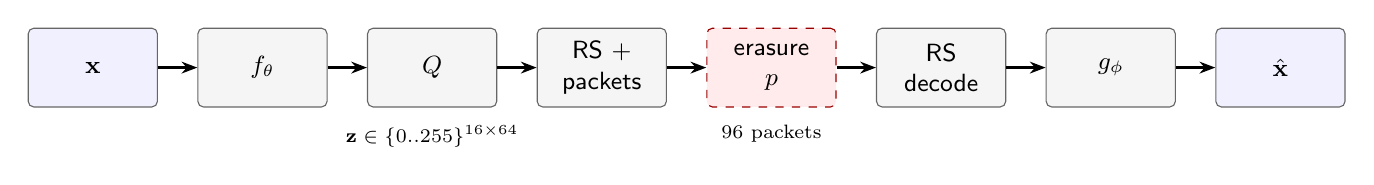
\begin{tikzpicture}[font=\sffamily\small, >={Stealth[length=2mm]}, node distance=4mm and 5mm,
  b/.style={draw=black!60, fill=black!4, rounded corners=2pt, align=center, minimum height=10mm, text width=15mm, inner sep=2pt},
  c/.style={b, fill=red!8, draw=red!60!black, dashed}]
\node[b, fill=blue!6] (x) {$\mathbf{x}$};
\node[b, right=of x] (f) {$f_\theta$};
\node[b, right=of f] (q) {$Q$};
\node[b, right=of q] (e) {RS +\\packets};
\node[c, right=of e] (ch) {erasure\\$p$};
\node[b, right=of ch] (d) {RS\\decode};
\node[b, right=of d] (g) {$g_\phi$};
\node[b, fill=blue!6, right=of g] (xh) {$\hat{\mathbf{x}}$};
\foreach \a/\b in {x/f,f/q,q/e,e/ch,ch/d,d/g,g/xh} \draw[->, thick] (\a) -- (\b);
\node[below=1mm of q, font=\scriptsize] {$\mathbf{z}\in\{0..255\}^{16\times64}$};
\node[below=1mm of ch, font=\scriptsize] {96 packets};
\end{tikzpicture}}
\caption{System model. A source $\mathbf{x}$ (image, speech segment or text window) is encoded by
$f_\theta$, quantized to $16\times64$ bytes, protected with systematic RS codes in 96 packets, sent over a
packet-erasure channel and decoded by $g_\phi$.}
\label{fig:system}
\end{figure}

\subsection{Sources and the common latent interface}
The system model is shown in Fig.~\ref{fig:system}. A source sample $\mathbf{x}$ is mapped by an encoder
$f_\theta$ to a latent of $C=16$ channels with $S=64$ values each. Table~\ref{tab:modalities} lists the
three sources. Images are $3\times32\times32$ CIFAR-10 images \cite{krizhevsky2009cifar} (3,072 values,
bandwidth ratio $k/n=1/6$ in the convention of \cite{bourtsoulatze2019deep}); speech samples are
1.024~s segments of LibriSpeech \cite{panayotov2015librispeech} (8~kbit/s after quantization); text
samples are 2,048-character windows of text8 \cite{mahoney2011text8} (27-symbol alphabet, 4 bits per
character). The image encoder has five convolutional layers; the speech and text encoders are their
one-dimensional counterparts, the text encoder after a character embedding. Each modality has two model
families: ADJSCC-Q, the ADJSCC backbone \cite{xu2022adjscc} with an attention-feature module after every
layer, and DeepJSCC-Q, the same network with every attention module removed.

\begin{table}[t]\centering
\caption{Sources, models and the shared latent interface}\label{tab:modalities}
\resizebox{\columnwidth}{!}{%
\begin{tabular}{llll}\toprule
 & Image & Speech & Text\\\midrule
Dataset & CIFAR-10 (CIFAR-100, Kodak) & LibriSpeech & text8\\
Unit & $3{\times}32{\times}32$ image & 1.024~s segment & 2,048 characters\\
Encoder & 2-D conv, 5 layers & 1-D conv & char.\ embedding + 1-D conv\\
Families & ADJSCC-Q / DeepJSCC-Q & ADJSCC-Q-1D / DeepJSCC-Q-1D & ADJSCC-Q-text / DeepJSCC-Q-text\\
Latent & \multicolumn{3}{c}{$16$ channels $\times$ $64$ one-byte symbols $= 1{,}024$ bytes}\\
Rate & $k/n=1/6$ & 8~kbit/s & 4~bit/char\\
Training loss & MSE & \TBD{MSE on waveform?} & cross-entropy\\
Train / val / test & 40k / 10k / 10k & 40k / -- / 4,000 & 40k / -- / 2,441 windows\\
Quality metric & PSNR (dB) & SNR, SI-SDR (dB) & char.\ / word accuracy (\%)\\
Clean test quality & 30.9--32.4~dB & 6.4--6.7~dB & 64.6--69.2\%\\
\bottomrule\end{tabular}}
\end{table}

\subsection{Byte quantization}
Every latent value is mapped to the nearest of 256 learned scalar centres, so that one value is one byte
and one GF(256) RS symbol. During training the forward pass uses the hard assignment and gradients flow
through a soft assignment, $z_q = z_{\mathrm{soft}} + \mathrm{sg}(z_{\mathrm{hard}}-z_{\mathrm{soft}})$,
as in DeepJSCC-Q \cite{tung2022deepjsccq}; the temperature $\sigma_q$ is annealed from 1.0 to 0.05 over 50
epochs and the centres are initialized between the 1st and 99th percentiles of the latent. Unlike
DeepJSCC-Q, which maps to I/Q constellation points, the quantizer is one-dimensional because the target
is a byte stream. On the first image model quantization cost 0.5~dB (31.04 to 30.53~dB) and the final
model uses 179 of the 256 levels. An unrecoverable byte is replaced by $0$ in latent space before
decoding; the receiver never sees ground truth.

\subsection{Packets, Reed--Solomon layouts and the budget}
The transmitter sends $N=96$ packets of 16 bytes, i.e.\ 1,536 bytes per sample and 50\% overhead over the
1,024-byte latent. The latent is first sorted by an importance ranking $\pi$ (most damaging channel first).
Codewords are laid out \emph{column-wise}: each packet is one row and carries one symbol of every
codeword, so a lost packet costs every codeword exactly one erasure (Fig.~\ref{fig:layout}). A first
layout that filled consecutive packets with one codeword failed 81\% of codewords at 20\% loss; the
interleaved layout fails 0.07\%. We compare the following layout families:
\begin{itemize}
\item \emph{No RS}: the 64 data packets alone (the remaining 32 slots are unused).
\item \emph{Uniform}: one systematic RS(96,64) code per byte column, i.e.\ equal protection. It survives
any 32 lost packets (33\%).
\item \emph{Grouped tiers}: tier $i$ owns $n_i$ consecutive packets and holds $k_i$ data packets (whole
channels, four packets each), RS$(n_i,k_i)$-coded column-wise; $n_i=k_i$ means no parity and $n_i=0$
means the tier is not sent. The hand-designed scheme of earlier work in this line is
$\{(32,16),(48,32),(16,16)\}$, called 25/50/25 (top 25\% of channels at rate 1/2, middle 50\% at rate
2/3, bottom 25\% uncoded). We also evaluate 25/25/50, 50/25/25, 25/75, 50/50 and 75/25 splits.
\item \emph{PET}: column $j$ of all 96 packets is one RS$(96,K_j)$ codeword; data fill the strongest
columns first \cite{albanese1996pet}.
\item \emph{Truncation}: RS$(96,4m)$ over the $m$ highest-ranked channels; the other $16-m$ channels are
not sent.
\end{itemize}
Every sorted layout must tell the receiver the order; this costs one byte per channel for a per-sample
ranking and nothing for a static table stored in the decoder.

\begin{figure}[t]\centering
\figbox{\columnwidth}{Packet layout (redraw slides 4 and 9). Left: interleaved RS(96,64); one codeword
per byte column, a lost packet (red row) costs every codeword one erasure. Right: the same 96 packets as
hand tiers T1 RS(32,16) / T2 RS(48,32) / T3 (16,16), and as truncation RS($96,4m$) with $16-m$ channels
not sent.}
\caption{Interleaved packetization and the layout families compared at a fixed budget of 96 packets.}
\label{fig:layout}
\end{figure}

\subsection{Channel}
Packets are erased independently with probability $p\in[0,0.5]$; the receiver knows which packets are
missing. For bursty losses we use a Gilbert--Elliott channel \cite{gilbert1960capacity,elliott1963estimates}
with 1\% loss in the good state, 85\% in the bad state, mean burst lengths of 1 to 16 packets and average
loss 35\% or 45\%. All methods see the same loss realizations (Section~\ref{sec:setup}).

\subsection{Problem statement}
Given a trained encoder, quantizer and decoder and a budget of $N$ packets, the transmitter chooses a
ranking $\pi$ and a layout $\mathcal{L}=\{(n_i,k_i)\}$ with $\sum_i n_i=N$ to minimize the expected
distortion over the erasure pattern $\mathbf{e}$,
\begin{equation}
\min_{\pi,\ \mathcal{L}:\ \sum_i n_i = N}\ \mathbb{E}_{\mathbf{e}}\!\left[d\big(\mathbf{x},
g_\phi(\mathrm{Dec}_{\mathcal{L}}(\mathrm{Enc}_{\mathcal{L},\pi}(Q(f_\theta(\mathbf{x}))),\mathbf{e}))\big)\right],
\end{equation}
where $d$ is the MSE for images and speech and the character error for text. The network is fixed; only
the protection changes.

% =====================================================================================================
\section{Importance-Aware Reed--Solomon Protection}\label{sec:method}
% Tier 1. Opens with the workflow figure, as Sec. III of the Deep JSCC paper opens with its architecture.

\begin{figure*}[t]\centering
\resizebox{\textwidth}{!}{%
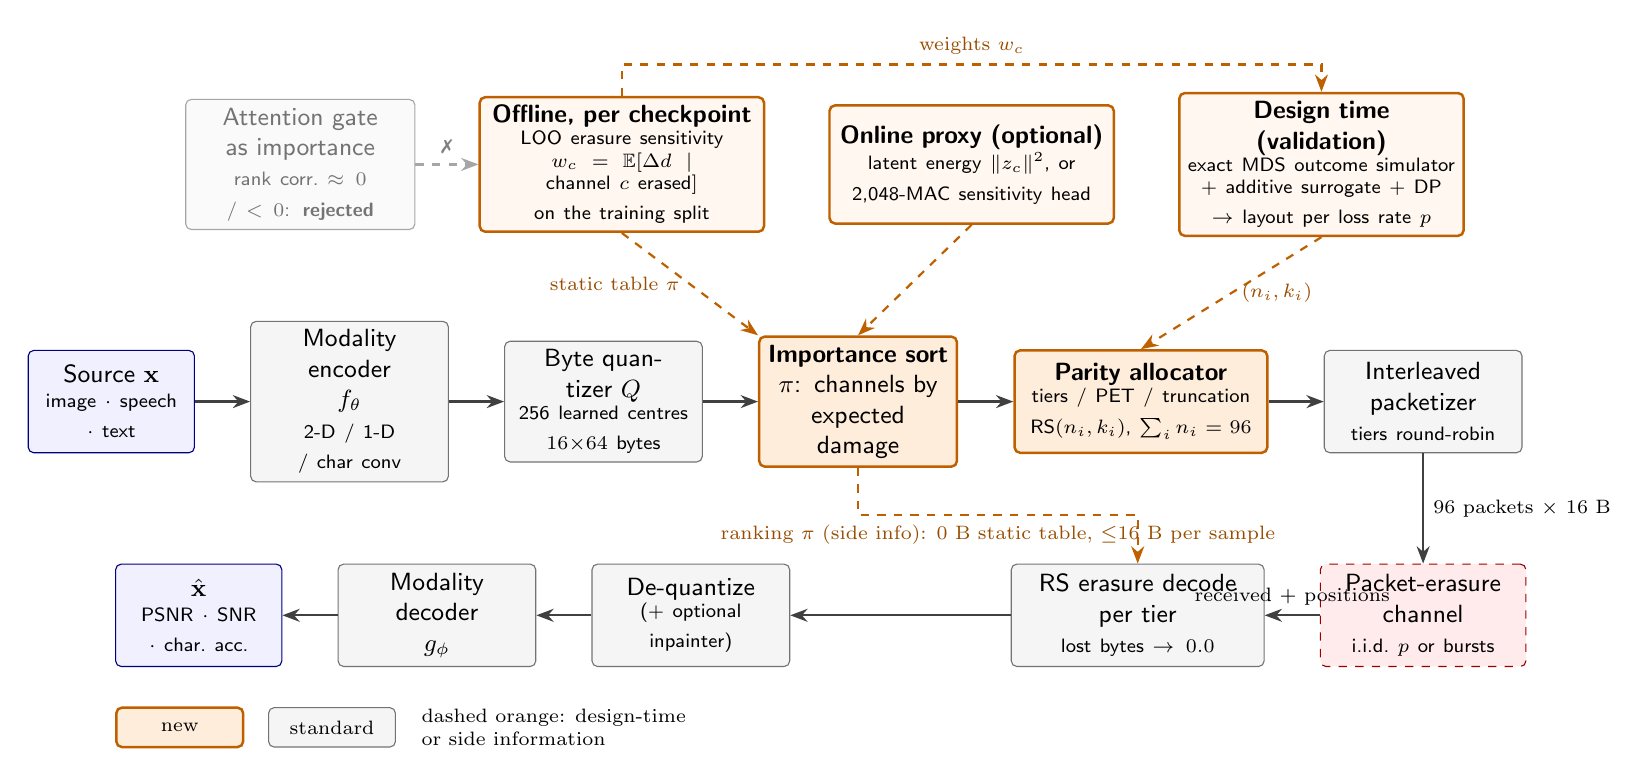
\begin{tikzpicture}[
  font=\sffamily\small, >={Stealth[length=2.2mm]}, node distance=6mm and 7mm,
  std/.style={draw=black!55, fill=black!4, rounded corners=2pt, align=center, minimum height=13mm,
              text width=23mm, inner sep=3pt},
  new/.style={std, draw=orange!75!black, fill=orange!14, line width=0.9pt},
  src/.style={std, text width=19mm, fill=blue!6, draw=blue!50!black},
  chan/.style={std, fill=red!8, draw=red!60!black, dashed, text width=24mm},
  off/.style={new, fill=orange!6, text width=34mm, minimum height=15mm},
  bad/.style={std, fill=black!2, draw=black!35, text=black!55, text width=27mm, minimum height=10mm},
  flow/.style={->, line width=0.8pt, draw=black!75},
  side/.style={->, line width=0.8pt, draw=orange!75!black, dashed}]

\node[src] (x) {Source $\mathbf{x}$\\[1pt]\scriptsize image $\cdot$ speech\\\scriptsize $\cdot$ text};
\node[std, right=of x] (enc) {Modality encoder\\$f_\theta$\\\scriptsize 2-D / 1-D / char conv};
\node[std, right=of enc] (q) {Byte quantizer $Q$\\\scriptsize 256 learned centres\\\scriptsize $16{\times}64$ bytes};
\node[new, right=of q] (sort) {\textbf{Importance sort}\\$\pi$: channels by\\expected damage};
\node[new, right=of sort, text width=30mm] (alloc) {\textbf{Parity allocator}\\\scriptsize tiers / PET / truncation\\\scriptsize RS$(n_i,k_i)$, $\sum_i n_i = 96$};
\node[std, right=of alloc] (pkt) {Interleaved\\packetizer\\\scriptsize tiers round-robin};

\node[chan, below=14mm of pkt] (ch) {Packet-erasure\\channel\\\scriptsize i.i.d.\ $p$ or bursts};

\node[std, left=of ch, text width=30mm] (rsdec) {RS erasure decode\\per tier\\\scriptsize lost bytes $\to 0.0$};
\node[std, left=of rsdec, xshift=-21mm] (deq) {De-quantize\\\scriptsize (+ optional\\\scriptsize inpainter)};
\node[std, left=of deq] (dec) {Modality decoder\\$g_\phi$};
\node[src, left=of dec] (xh) {$\hat{\mathbf{x}}$\\[1pt]\scriptsize PSNR $\cdot$ SNR\\\scriptsize $\cdot$ char.\ acc.};

\node[off, above=13mm of sort, xshift=-30mm] (loo) {\textbf{Offline, per checkpoint}\\\scriptsize LOO erasure sensitivity\\\scriptsize $w_c=\mathbb{E}[\Delta d \mid \text{channel } c \text{ erased}]$\\\scriptsize on the training split};
\node[off, right=8mm of loo] (proxy) {\textbf{Online proxy (optional)}\\\scriptsize latent energy $\|z_c\|^2$, or\\\scriptsize 2,048-MAC sensitivity head};
\node[off, right=8mm of proxy] (sim) {\textbf{Design time (validation)}\\\scriptsize exact MDS outcome simulator\\\scriptsize + additive surrogate + DP\\\scriptsize $\to$ layout per loss rate $p$};
\node[bad, left=8mm of loo] (att) {Attention gate as importance\\\scriptsize rank corr.\ $\approx 0$ / $<0$: \textbf{rejected}};

\draw[flow] (x) -- (enc);
\draw[flow] (enc) -- (q);
\draw[flow] (q) -- (sort);
\draw[flow] (sort) -- (alloc);
\draw[flow] (alloc) -- (pkt);
\draw[flow] (pkt) -- node[right, font=\scriptsize] {96 packets $\times$ 16 B} (ch);
\draw[flow] (ch) -- node[above, font=\scriptsize] {received + positions} (rsdec);
\draw[flow] (rsdec) -- (deq);
\draw[flow] (deq) -- (dec);
\draw[flow] (dec) -- (xh);

\draw[side] (loo.south) -- node[left, font=\scriptsize, text=orange!60!black] {static table $\pi$} (sort.north west);
\draw[side] (proxy.south) -- (sort.north);
\draw[side] (sim.south) -- node[right, font=\scriptsize, text=orange!60!black] {$(n_i,k_i)$} (alloc.north);
\draw[side] (loo.north) |- ++(0,4mm) -| node[pos=0.25, above, font=\scriptsize, text=orange!60!black] {weights $w_c$} (sim.north);
\draw[->, line width=0.8pt, draw=black!35, dashed] (att.east) -- node[above, font=\scriptsize, text=black!50] {\ding{55}} (loo.west);

\draw[side] (sort.south) -- ++(0,-6mm) -| node[pos=0.25, below, font=\scriptsize, text=orange!60!black]
      {ranking $\pi$ (side info): 0 B static table, $\le$16 B per sample} (rsdec.north);

\node[new, text width=14mm, minimum height=5mm, below=5mm of xh.south west, anchor=north west, font=\scriptsize] (l1) {new};
\node[std, text width=14mm, minimum height=5mm, right=3mm of l1, font=\scriptsize] (l2) {standard};
\node[right=2mm of l2, font=\scriptsize, align=left] {dashed orange: design-time\\or side information};
\end{tikzpicture}}
\caption{The proposed pipeline. Standard deep-JSCC blocks are grey. The blocks specific to this work are
orange: an offline leave-one-out sensitivity table per checkpoint (or a cheap online proxy) sorts the
latent channels, and an allocator, designed with an exact MDS simulator, spends a fixed budget of 96
packets on tiered RS codes or truncation. The same interface serves image, speech and text models. The
attention gates of the backbone, a common importance signal in prior work, are not used: they do not rank
erasure damage in any modality (Section~\ref{sec:res-cross}).}
\label{fig:workflow}
\end{figure*}

Fig.~\ref{fig:workflow} shows the pipeline. Four components are specific to this work: a measurement of
what ``important'' means for a given checkpoint, cheap predictors of it, an exact model of the RS
receiver, and an allocator that uses both.

\subsection{Erasure sensitivity: what ``important'' means}
For a trained model we erase one latent channel $c$ at a time (its 64 bytes are set to $0$), decode, and
record the increase of the distortion, $\Delta d_c(\mathbf{x})$. Averaging over the training split gives
the LOO profile $w_c=\mathbb{E}_{\mathbf{x}}[\Delta d_c(\mathbf{x})]$ and a static ranking $\pi$ that sorts
$w_1\ge\dots\ge w_{16}$. We summarize a profile by two numbers used for every modality: the \emph{top-4
share}, the fraction of the total LOO damage (in dB for images and speech, in percentage points for
text) carried by the four most damaging channels, which equals 25\% for a flat profile, and the
worst-channel damage. \TBD{Fix one definition of top-4 share for all modalities (dB share used here; the
GLOBECOM draft used MSE share, 66--84\%).} The per-sample damage $\Delta d_c(\mathbf{x})$ is also the
ground truth against which every predictor is scored.

\subsection{Predicting sensitivity without an oracle}
The LOO profile needs one decoder pass per channel. A transmitter can instead use: (a) the static table
of the checkpoint, which costs no side information when stored in the decoder; (b) per-sample latent
statistics, namely energy $\|z_c\|_2^2$, $\ell_1$ norm, variance and a first-order Taylor saliency
$|\nabla_{z_c} d\cdot z_c|$; (c) a learned \emph{sensitivity head}, a two-layer MLP of 2,048
multiply-accumulates on pooled latent statistics, trained to regress $\Delta d_c(\mathbf{x})$ on the
training split; or (d) the attention gate of the bottleneck module, which pools each channel, appends the
SNR, and outputs one sigmoid weight per channel \cite{xu2022adjscc}. Predictors are scored by the
within-sample Spearman correlation with the true damage, the overlap of their top four channels with
the true top four (0.25 by chance), and the \emph{protection regret}, the true damage of the channels a
predictor leaves unprotected minus that of the oracle.

The attention gates are a natural candidate, and prior work uses them that way, but they are trained to
rescale channels against additive noise of a given SNR. Nothing in that objective measures what losing
an entire channel costs; Section~\ref{sec:res-cross} shows that the two are unrelated.

\subsection{Exact receiver outcome for systematic MDS layouts}
\begin{lemma}[Exact outcome]\label{lem:exact}
For a systematic MDS code used for erasure decoding, a data byte is lost if and only if its packet is
erased and its codeword has more than $n-k$ erased symbols. The set of lost latent bytes is therefore a
deterministic function of the erasure pattern and the layout. Under i.i.d.\ loss with rate $p$, a data
byte of an RS$(n,k)$ codeword is lost with probability
\begin{equation}
q(n,k,p) \;=\; p\;\Pr\!\left[\mathrm{Bin}(n-1,p)\ge n-k\right]. \label{eq:q}
\end{equation}
\end{lemma}
\begin{proof}
An MDS code recovers any $k$ of its $n$ symbols. If decoding fails, a systematic code still delivers its
received data symbols. A given data byte is therefore lost iff its own packet is erased and at least
$n-k$ of the other $n-1$ packets are erased, which gives \eqref{eq:q}.
\end{proof}
We verified Lemma~\ref{lem:exact} symbol by symbol against a GF(256) RS decoder for every layout family.
It replaces RS decoding in simulation by a mask product, so evaluating a layout costs one decoder pass,
and the simulator reproduces the RS-decoded sweep of the primary image model to within
\ReferenceMaxDiff~dB on \ReferenceCells{} cells.

\subsection{Allocating a fixed parity budget}
Let $w_r$ be the LOO weight of the channel of rank $r$ and assume that damage adds up over lost bytes.
With $\mathcal{T}$ the set of codewords and $W(c)$ the total weight of the data bytes of codeword $c$,
\begin{equation}
\mathbb{E}[d] \;\approx\; d_0 + \sum_{c\in\mathcal{T}} W(c)\, q(n_c,k_c,p)
\;+\; \sum_{r\ \text{not sent}} w_r . \label{eq:surrogate}
\end{equation}
For grouped tiers and for PET, \eqref{eq:surrogate} is separable over consecutive segments of the sorted
stream, so its minimum over all allocations with $N$ packets follows exactly from a dynamic program over
(channels placed, packets used), at cost $O(C^2N^2)$ for grouped tiers. Because additivity is only
approximate, candidates are re-scored with the exact simulator on the validation split and refined by
local search. We also simulate the 25 surrogate-best allocations with two or three tiers to check whether
a genuinely multi-level code ever beats single-code designs.

\begin{proposition}[When truncation beats equal protection]\label{prop:trunc}
Under \eqref{eq:surrogate}, sending the top $m$ channels with RS$(N,4m)$ beats uniform RS$(N,64)$ iff
\begin{equation}
\textstyle\sum_{r>m} w_r \;<\; q(N,64,p)\sum_{r} w_r \;-\; q(N,4m,p)\sum_{r\le m} w_r .
\end{equation}
\end{proposition}
The right-hand side is the protection bought by spending $4(16-m)$ more packets on parity; the left-hand
side is the damage of the channels left out, which is small only if the ranking puts the truly least
damaging channels last. A random order makes it about $(16-m)/16$ of the total damage; an accurate order
makes it the smallest tail of the profile. The coding gain of truncation is therefore governed by the
concentration of the profile \emph{and} the quality of the ranking, which is what the cross-modal
experiments test.

\subsection{Bursts, side information and complexity}
Under bursty loss, tiers sent one after another let a single burst erase a whole tier. We therefore
interleave the packets of all tiers round-robin. Side information is 0~B with a static table (16~B with a
per-sample ranking). The sensitivity head costs 2,048 MACs, 0.039\% of the image encoder and 0.024\% of
the speech encoder. The receiver runs the same RS decoder as for uniform protection.

% =====================================================================================================
\section{Experimental Setup}\label{sec:setup}
% Tier 1/2 (protocol credibility).
\subsection{Datasets and splits}
\emph{Images.} CIFAR-10 split 40k/10k/10k (train/validation/test); models and LOO tables use the
training split, scheme selection the validation split, and the test split is used once for the reported
numbers (every access is logged). CIFAR-100 tests the transfer of the ranking; the 24 Kodak images
\cite{kodak} ($768\times512$) test larger inputs with the CIFAR model (packet size 128~B; relative results
only, clean 24.3~dB). \emph{Speech.} LibriSpeech \cite{panayotov2015librispeech}, 1.024~s segments, 40k
training segments, 4,000 test segments per channel seed. \emph{Text.} text8 \cite{mahoney2011text8}
(100M characters, 27 symbols), non-overlapping 2,048-character windows from disjoint train/validation/test
character ranges, 40k training windows, 2,441 test windows.

\subsection{Models and training}
All models are trained over an identity channel (images: MSE; text: cross-entropy; \TBD{speech loss}),
with the annealed quantizer, for 60 epochs. Seeds: ADJSCC-Q images 6 (seeds 42, 100, 7, 13, 21, 2024),
DeepJSCC-Q images 4 (42, 100, 13, 7) \TBD{reconcile with the DeepJSCC-Q set 100/21/7 of the GLOBECOM
tables}, ADJSCC-Q-1D 3 (42, 100, 7), DeepJSCC-Q-1D 4 (42, 100, 13, 7), ADJSCC-Q-text 3, DeepJSCC-Q-text 3.
A convergence rule fixed before evaluation excludes models whose best validation epoch is below 50. It
excludes ADJSCC-Q image seed 2024 (clean 26.5~dB), DeepJSCC-Q-1D seed 100, all three ADJSCC-Q-text models
(clean 42.6--44.0\%) and DeepJSCC-Q-text seed 100 (43.8\%). Unquantized ADJSCC reaches 22.01, 25.23,
27.85, 29.32 and 29.92~dB on CIFAR-10 at 0, 5, 10, 15 and 20~dB AWGN SNR, matching \cite{xu2022adjscc}.
The primary image model (ADJSCC-Q seed 42) has a clean test PSNR of \CleanPsnr~dB.

\subsection{Evaluation protocol}
One master loss mask is drawn per (batch, channel seed, loss rate) and shared by all methods; smaller
schemes use its first columns. Results use five channel seeds; we report the mean over seeds with the
95\% $t$-interval, and gains are paired differences against uniform RS on identical losses. Every result
file stores the commit and the checkpoint hash. Scheme choice and truncation depth are made on
validation. For speech and text we pre-registered three criteria before running the test sweeps:
\textbf{C1} the family's mean top-4 share is at least 40\%; \textbf{C2} every model's LOO-ranked gain at
40\% loss is at least $+1.5$~dB (speech) or $+2.0$\pp{} (text) with a confidence interval above zero;
\textbf{C3} a random order gets less than half of the LOO gain for loss $\ge35\%$. A family that misses
C1 with a top-4 share below 30\% and an LOO--random gap of at most 0.5 is labelled FLAT.

\subsection{Baselines}
No RS; uniform RS(96,64); hand-designed tiers with LOO, per-sample LOO, energy, $\ell_1$, head, random and
attention orders; the PET twin of the hand tiers; an unsorted two-tier control with two RS(48,32) blocks
(isolating block length); a uniform PET layout; Grad-FEC-style drop-and-protect \cite{uyanik2023gradfec};
optimized grouped, PET and truncation layouts; models trained for fewer channels; nested-dropout ordered
models; a 24-channel JSCC that spends all 1,536 bytes on latent symbols without RS, fine-tuned over
erasures; and JPEG, JPEG2000 and WebP at the same 1,024-byte budget with fixed RS(96,64) or with
validation-chosen rate adaptation (fewer source bytes, stronger code).

\subsection{Metrics}
Images: PSNR. The SSIM implementation of the code base uses zero-padded windows, so we report PSNR only.
Speech: per-segment SNR and SI-SDR \cite{leroux2019sdr}. \TBD{PESQ-WB and STOI were not computed;
compute or drop.} Text: per-window character accuracy and word accuracy. Gains are differences in the
native unit (dB, or percentage points for text).

% =====================================================================================================
\section{Results}\label{sec:results}

% -----------------------------------------------------------------------------------------------------
\subsection{Images}\label{sec:res-img}

\subsubsection{Erasure sensitivity is concentrated, with or without attention}
% Tier 1. published_results/gpu/phase1/multiseed/multiseed.md; results/g1/deepjsccq/multiseed/multiseed.md
Fig.~\ref{fig:img-profiles} and Table~\ref{tab:profiles} show the sorted LOO profiles. In the five
converged ADJSCC-Q models the four most damaging of 16 channels carry 45--53\% of the damage, against
25\% for a flat profile. The worst channel costs 8.7--17.1~dB and the least damaging 0.9--2.2~dB. The
sorted profiles agree across seeds (mean Pearson correlation 0.922, mean absolute difference
0.83~dB per channel) although the channel indices permute (index-aligned Spearman $-0.13$): the
ranking belongs to a checkpoint, the shape of the profile to the architecture and the data. DeepJSCC-Q,
which has no attention module, is also concentrated (top-4 share 33--40\%, every seed with a channel above
10~dB, profile Pearson 0.930), so the inequality is not created by the gates. The CIFAR-10 table of the
primary model transfers to CIFAR-100 with Spearman 0.997, Kendall 0.983 and identical top four.

\begin{figure}[t]\centering
\resfig{\columnwidth}{fig_profiles.pdf}{Sorted LOO damage profiles, ADJSCC-Q and DeepJSCC-Q}
\caption{Sorted share of LOO damage per latent channel, CIFAR-10 (thin: training seeds; thick: mean).
Both architectures concentrate damage far above the equal share.}\label{fig:img-profiles}
\end{figure}

\begin{table}[t]\centering
\caption{LOO sensitivity profiles of all converged models (damage in dB; text in pp)}\label{tab:profiles}
\resizebox{\columnwidth}{!}{%
\begin{tabular}{llcccc}\toprule
Modality & Model & Seeds & Top-4 share & Worst ch. & Least ch.\\\midrule
Image & ADJSCC-Q & 5 & 45--53\% & 8.7--17.1 & 0.9--2.2\\
Image & DeepJSCC-Q & 4 & 33--40\% & 10.5--11.7 & 0.3--4.4\\
Speech & ADJSCC-Q-1D & 3 & 38--46\% & 5.2--9.8 & 1.4\\
Speech & DeepJSCC-Q-1D & 3 & 46--48\% & 9.4--11.7 & 1.4--1.6\\
Text & DeepJSCC-Q-text & 2 & 28--30\% & 24.6--31.1 & 12.4--15.9\\\midrule
\multicolumn{6}{l}{\footnotesize Profile Pearson across seeds: 0.92, 0.93, 0.97, 0.83, 0.90 (same order).}\\
\bottomrule\end{tabular}}
\end{table}

\subsubsection{Which predictor ranks it}
% Tier 1/2. published_results/gpu/phase1/{saliency,head,transfer}; results/g1/deepjsccq/seed42/{saliency,head}
Table~\ref{tab:proxies} scores every predictor against the true per-image damage. For ADJSCC-Q the
bottleneck attention gate has a within-image Spearman correlation of $-0.015$ (95\% CI $-0.020$ to
$-0.011$) and a top-4 overlap of 0.23, below the 0.25 of a random pick (Fig.~\ref{fig:img-att}); pooled
over images the Pearson correlation is $+0.118$ because gate levels and damage both vary between
channels, but within an image the gate does not order them. The static training table reaches $+0.89$,
energy and $\ell_1$ $+0.84$, the Taylor proxy $+0.63$ and variance $+0.44$. The 2,048-MAC head reaches a
top-4 overlap of 0.92 ($\pm0.001$ over five head seeds) and a protection regret of 0.21~dB per image,
against 0.60~dB for the static table and 15.9~dB for a random order. For DeepJSCC-Q the static table is
weaker ($+0.74$, regret 2.30~dB), energy is unchanged ($+0.84$) and the head again closes most of the gap
(0.88 overlap, 0.34~dB regret).

\begin{figure}[t]\centering
\resfig{\columnwidth}{eval/oracle_attention_correlation.png}{Attention gate vs LOO damage scatter}
\caption{Attention gate value versus PSNR drop when that channel is lost (CIFAR-10, ADJSCC-Q, 2,000
images $\times$ 16 channels). Pooled Pearson $+0.118$; within an image, Spearman $-0.015$.}\label{fig:img-att}
\end{figure}

\subsubsection{The ranking, not the tiering, makes the gain}
% Tier 1. published_results/gpu/report/headline.md, coding_controls_test.md
Table~\ref{tab:img-headline} and Fig.~\ref{fig:img-main} report the primary model on the full test
split. Uniform RS(96,64) is lossless up to 20\% loss, loses 2.2~dB at 30\%, and falls off its cliff
($-4.27$~dB between 30 and 35\%) to 20.73~dB at 40\%. Without RS the quality drops from the first lost
packet (25.80~dB at 10\%). The hand-designed 25/50/25 tiers overtake uniform RS from about 32\% loss and
gain $+2.86$~dB at 40\% with the static LOO order; energy ($+2.92$), $\ell_1$ ($+2.89$) and the head
($+3.00$, 95\% CI $\pm0.03$) match it, and a per-image LOO order, which no transmitter can compute, adds
only 0.2~dB ($+3.08$). The same tiers with a random order gain $+0.94$~dB and with attention order
$+0.74$~dB. Averaged over loss $\ge35\%$ with the best scheme per ranking, the gains are head $+2.31$,
energy $+2.24$, $\ell_1$ $+2.22$, LOO $+2.19$, random $+0.50$ and attention $+0.31$~dB: a random order
recovers 23\% of the LOO gain and attention 14\%. Same tiers, same 96 packets: only the channel order
changes. Below the crossover the fixed scheme pays for its unprotected bottom tier ($-0.95$~dB at 30\%,
$-1.19$ at 20\%). The tail improves with the mean: the 5th-percentile PSNR at 40\% rises from 16.66 to
18.74~dB.

\begin{table*}[t]\centering
\caption{Primary image model (ADJSCC-Q, CIFAR-10 test, $10{,}000$ images $\times$ 5 channel seeds): PSNR of
uniform RS and no RS (dB) and paired gain of the hand-designed 25/50/25 tiers over uniform RS (dB) for each ranking}
\label{tab:img-headline}
\begin{tabular}{lcccccccccc}\toprule
Loss & uniform & no RS & LOO & per-image LOO & energy & $\ell_1$ & head & random & attention & PET twin\\\midrule
0.10 & 30.88 & 25.80 & $-0.61$ & $-0.53$ & $-0.58$ & $-0.60$ & $-0.58$ & $-1.74$ & $-1.47$ & $-0.67$\\
0.20 & 30.88 & 23.09 & $-1.19$ & $-1.06$ & $-1.17$ & $-1.19$ & $-1.15$ & $-3.15$ & $-2.77$ & $-1.25$\\
0.30 & 28.67 & 21.16 & $-0.95$ & $-0.77$ & $-0.92$ & $-0.95$ & $-0.87$ & $-3.33$ & $-3.10$ & $-0.41$\\
0.35 & 24.40 & 20.36 & $+1.31$ & $+1.52$ & $+1.36$ & $+1.33$ & $+1.42$ & $-0.93$ & $-0.93$ & $+1.53$\\
0.40 & 20.73 & 19.62 & $+2.86$ & $+3.08$ & $+2.92$ & $+2.89$ & $+3.00$ & $+0.94$ & $+0.74$ & $+2.78$\\
0.45 & 19.07 & 18.94 & $+2.69$ & $+2.90$ & $+2.76$ & $+2.73$ & $+2.83$ & $+1.17$ & $+0.88$ & $+2.93$\\
0.50 & 18.31 & 18.31 & $+1.89$ & $+2.05$ & $+1.94$ & $+1.92$ & $+2.00$ & $+0.81$ & $+0.55$ & $+2.37$\\
\bottomrule\end{tabular}
\end{table*}

\begin{figure}[t]\centering
\resfig{\columnwidth}{fig_main.pdf}{PSNR vs loss: uniform, hand-tiered, optimized truncation, ordered model, WebP}
\caption{Test PSNR versus packet loss rate, images (1,536 transmitted bytes per image). Optimized
allocations are chosen per loss rate on validation.}\label{fig:img-main}
\end{figure}

\subsubsection{Other tier shapes and the block-length control}
% Tier 3/4. published_results/gpu/final/final_test.md
The other hand-designed splits trace the same trade-off (primary model, LOO order, gain at 30/40/50\%):
25/25/50 $-2.31/+2.70/+1.99$; 25/75 $-3.14/+1.91/+1.85$; 75/25 $-5.26/-0.61/+0.27$; 50/50
$-1.16/+0.46/+0.09$~dB. Protecting a small top tier strongly is what pays at high loss. The unsorted
control with two RS(48,32) blocks at the uniform rate gains \TwoTierUnsortedGainForty~dB at 40\% and
\TwoTierUnsortedGainThirty~dB at 30\%: shorter blocks alone do not help. A uniform PET layout with
diagonal interleaving gains \UniformDiagGainForty~dB at 40\%.

\subsubsection{The optimal allocation is importance-ordered truncation}
% Tier 1. published_results/coding/seed42/coding_controls_test.md, macros.
Table~\ref{tab:alloc} reports the validation-optimized designs. Up to 20\% loss the search returns
uniform RS. From 30\% on it returns truncation, keeping the top \TruncKeepThirty, \TruncKeepThirtyFive,
\TruncKeepForty, \TruncKeepFortyFive{} and \TruncKeepFifty{} channels at 30, 35, 40, 45 and 50\% loss, each in one
RS$(96,4m)$ block, or a PET or multi-tier layout within a few tenths of a dB of it. The 25
surrogate-best genuinely multi-tier allocations improve on truncation by at most \MultiTierMaxGain~dB on
validation, and optimized PET designs are within \PetVsTruncMax~dB. On the test split, truncation in LOO
order gains \TruncOracleGainForty~dB at 40\% loss (\TruncOracleForty~dB against \UniformForty~dB) and
\TruncOracleGainFifty~dB at 50\%, \TruncOverHandForty~dB more than the hand-designed tiers, and it is never
worse than uniform RS at low loss, because there the selected design \emph{is} uniform RS. A selector that
signals one byte per change of the loss rate reaches \SelectorGainForty~dB at 40\% and
\SelectorGainFortyFive~dB at 45\%.

The ranking now decides almost everything. With the same validation-chosen depth, truncation in random
order gains only \TruncRandomGainForty~dB at 40\% loss, in attention order \TruncAttentionGainForty~dB,
in energy order \TruncEnergyGainForty~dB and with the head \TruncHeadGainForty~dB.
Proposition~\ref{prop:trunc} explains why: the coding gain of truncation is paid for by the channels
left out. Attention order is erratic rather than uniformly bad: it gains \TruncAttentionGainThirtyFive~dB
at 35\% but only \TruncAttentionGainFortyFive~dB at 45\% and \TruncAttentionGainFifty~dB at 50\%, when
the truncation cuts deeper into channels it ranks wrongly. Grad-FEC-style drop-and-protect (top eight
channels coded, four dropped) gains \GradFecGainForty~dB at 40\% but costs \GradFecGainZero~dB on a
clean channel; the selector avoids that cost.

The additive surrogate~\eqref{eq:surrogate} predicts the simulated mean MSE of the test-evaluated layouts
with Spearman correlation \SurrogateSpearman{} and median relative error \SurrogateMedianRelErr\%
(Fig.~\ref{fig:surrogate}). It underestimates the MSE when many channels are partly lost at once, because
damage is mildly superadditive, but it ranks layouts well; the final choice is always made by exact
simulation.

\begin{table}[t]\centering\caption{Test PSNR (dB) and gain over uniform RS at 40\% loss, primary image model}\label{tab:alloc}
\begin{tabular}{lrr}\toprule
Method & PSNR & gain\\\midrule
uniform RS(96,64) & \UniformForty & --\\
no RS (64 packets, 32 idle) & \NoRSForty & \NoRSGainForty\\
unsorted 2 $\times$ RS(48,32) & \TwoTierUnsortedForty & \TwoTierUnsortedGainForty\\
uniform PET (diagonal) & \UniformDiagForty & \UniformDiagGainForty\\
hand-tiered 25/50/25, LOO order & \HandTierForty & \HandTierGainForty\\
hand-tiered 25/50/25, per-image LOO & \HandTierPerImageForty & \HandTierPerImageGainForty\\
hand-tiered 25/50/25, random order & \HandTierRandomForty & \HandTierRandomGainForty\\
hand-tiered 25/50/25, attention order & \HandTierAttentionForty & \HandTierAttentionGainForty\\
PET twin of 25/50/25 & \PetTwinForty & \PetTwinGainForty\\
Grad-FEC style (top 8 coded, 4 dropped) & \GradFecForty & \GradFecGainForty\\
opt.\ truncation, random order & \TruncRandomForty & \TruncRandomGainForty\\
opt.\ truncation, attention order & \TruncAttentionForty & \TruncAttentionGainForty\\
opt.\ truncation, energy order & \TruncEnergyForty & \TruncEnergyGainForty\\
opt.\ truncation, 2,048-MAC head & \TruncHeadForty & \TruncHeadGainForty\\
opt.\ truncation, LOO order & \TruncOracleForty & \TruncOracleGainForty\\
opt.\ grouped (multi-tier allowed) & \OptGroupedForty & \OptGroupedGainForty\\
opt.\ PET & \OptPetForty & \OptPetGainForty\\
selector (per loss rate) & \SelectorForty & \SelectorGainForty\\\bottomrule
\end{tabular}\end{table}

\begin{figure}[t]\centering
\resfig{\columnwidth}{fig_surrogate.pdf}{Surrogate vs simulated MSE}
\caption{Additive surrogate~\eqref{eq:surrogate} versus simulated mean MSE for every LOO-ordered layout
and loss rate evaluated on the test split.}\label{fig:surrogate}
\end{figure}

\subsubsection{Unknown loss rate}
% Tier 2. coding_controls_test.md (design0.x, robust_*), fig_mismatch.
An allocation is only optimal at the loss rate it was designed for (Fig.~\ref{fig:mismatch}). A
truncation designed for 40\% gives up \DesignFortyAtZeroLoss~dB on a clean channel and gains
\DesignFortyAtFifty~dB at 50\%; one designed for 35\% gives up 1.59~dB clean and gains 5.87~dB at 40\%.
A single allocation optimized over $p\in[0.1,0.5]$ changes the PSNR by \RobustGroupedGainTen~dB at 10\%
and \RobustGroupedGainForty~dB at 40\%. This is the only regime in which the search selects a multi-level
structure (robust PET: \RobustPetGainTen~dB at 10\%, \RobustPetGainForty~dB at 40\%). With loss-rate
feedback, the selector of Table~\ref{tab:alloc} is the operating point we recommend.

\begin{figure}[t]\centering
\resfig{\columnwidth}{fig_mismatch.pdf}{Design-rate mismatch}
\caption{Gain over uniform RS of allocations designed for one loss rate and used at another.}\label{fig:mismatch}
\end{figure}

\subsubsection{Replication across seeds and architectures}
% Tier 2. published_results/gpu/multiseed/*, results/g1/deepjsccq/*, paper/generated_tables.tex
Table~\ref{tab:img-seeds} repeats the hand-tiered comparison for every converged image model. ADJSCC-Q
gains $+2.35$ to $+3.11$~dB at 40\% with the LOO order and $+2.07$ to $+3.23$ with energy, while
attention ranges from $-0.33$ to $+0.74$~dB. The four DeepJSCC-Q models gain $+2.05$ to $+2.76$~dB with
LOO and only $+0.56$ to $+0.64$ with a random order; their low-loss penalty is larger ($-1.96$ to
$-3.82$~dB at 30\%), because without attention their uniform-RS operating point is higher (clean
31.5--32.4~dB) and their unprotected channels cost more. Table~\ref{tab:seeds} repeats the optimal
truncation for every converged model: LOO-ordered truncation gains \TruncGainMinAdj{} to
\TruncGainMaxAdj~dB at 40\% for ADJSCC-Q and \TruncGainMinDeep{} to \TruncGainMaxDeep~dB for DeepJSCC-Q,
beating the hand-tiered scheme on every model by \TruncOverHandMinAll{} to \TruncOverHandMaxAll~dB.
Energy order is within 0.9~dB of LOO order on every model, while attention order ranges from below the
random order (ADJSCC-Q seed 21) to 1.5~dB under LOO order.

\begin{table}[t]\centering
\caption{Hand-tiered 25/50/25 on every converged image model: gain over uniform RS (dB)}\label{tab:img-seeds}
\resizebox{\columnwidth}{!}{%
\begin{tabular}{llccccccc}\toprule
Model & seed & clean & unif.\ @40 & LOO @40 & energy @40 & random @40 & attn.\ @40 & LOO @30\\\midrule
ADJSCC-Q & 42 & 30.88 & 20.73 & $+2.86$ & $+2.92$ & $+0.94$ & $+0.74$ & $-0.95$\\
ADJSCC-Q & 100 & 31.34 & 20.77 & $+2.83$ & $+2.76$ & -- & $+0.54$ & $-1.52$\\
ADJSCC-Q & 13 & 31.76 & 20.64 & $+2.90$ & $+3.23$ & -- & $-0.33$ & $-1.55$\\
ADJSCC-Q & 21 & 31.09 & 20.79 & $+3.11$ & $+2.07$ & -- & $-0.05$ & $-1.09$\\
ADJSCC-Q & 7 & 31.45 & 21.02 & $+2.35$ & $+2.59$ & -- & $+0.42$ & $-1.82$\\
DeepJSCC-Q & 42 & 32.38 & 19.00 & $+2.11$ & $+2.05$ & $+0.62$ & -- & $-3.82$\\
DeepJSCC-Q & 100 & 31.54 & 18.34 & $+2.05$ & $+1.77$ & $+0.56$ & -- & $-3.67$\\
DeepJSCC-Q & 13 & 32.40 & 18.96 & $+2.43$ & $+2.54$ & $+0.64$ & -- & $-2.93$\\
DeepJSCC-Q & 7 & 31.66 & 18.58 & $+2.76$ & $+2.78$ & $+0.62$ & -- & $-1.96$\\
\bottomrule\end{tabular}}
\end{table}

\begin{table}[t]\centering\caption{Optimal truncation at 40\% loss across image models: test PSNR (dB)
\TBD{DeepJSCC-Q rows are the GLOBECOM set (seeds 100/21/7); reconcile with Table~\ref{tab:img-seeds}}}\label{tab:seeds}
\resizebox{\columnwidth}{!}{\IfFileExists{../paper/generated_tables.tex}{% generated by experiments/paper_figures.py -- do not edit
\begin{tabular}{lrrrrrrr}
\toprule
model & clean & uniform & hand-tiered & \multicolumn{4}{c}{opt.\ truncation, order:} \\
 & & & LOO & LOO & energy & attention & random \\
\midrule
ADJSCC-Q s100 & 31.34 & 20.77 & 23.60 & 25.77 & 25.75 & 23.15 & 22.28 \\
ADJSCC-Q s13 & 31.76 & 20.64 & 23.54 & 26.18 & 26.36 & 22.41 & 22.13 \\
ADJSCC-Q s21 & 31.09 & 20.79 & 23.90 & 26.14 & 25.27 & 20.78 & 22.24 \\
ADJSCC-Q s42 & 30.88 & 20.73 & 23.59 & 27.25 & 26.72 & 25.72 & 22.42 \\
ADJSCC-Q s7 & 31.45 & 21.02 & 23.37 & 25.04 & 25.74 & 23.25 & 22.70 \\
DeepJSCC-Q s100 & 31.79 & 18.56 & 22.19 & 28.00 & 27.89 & -- & 20.54 \\
DeepJSCC-Q s21 & 32.73 & 19.52 & 22.70 & 25.63 & 26.03 & -- & 21.51 \\
DeepJSCC-Q s7 & 32.17 & 17.81 & 21.86 & 26.03 & 26.08 & -- & 19.64 \\
\bottomrule
\end{tabular}
}{\TBD{generated\_tables.tex}}}
\end{table}

\subsubsection{Ordered latents and smaller models}
% Tier 2. macros Ordered*, KnTwelve*, KnSixteen*.
Truncating a 16-channel model to $m$ channels competes with a model trained for $m$ channels. With the
same 96 packets, the 8-channel model ($k/n=1/12$) behind RS(96,32) gives \KnTwelveClean~dB at every loss
rate up to 50\%, because its code essentially never fails, and the 6-channel model behind RS(96,24) gives
\KnSixteenForty~dB. Switching between such models dominates truncation of an unordered model at high
loss; truncation is the single-model approximation to this envelope, and its quality is set by the
ranking. Nested (tail) dropout \cite{rippel2014nested} closes the gap with one network: during training
half of the images keep only a uniformly random prefix of the 16 channels. The LOO order of the resulting
model equals the channel index, the last five channels each cost at most 0.02~dB, and the clean cost is
\OrderedCleanCost~dB. Truncation in index order then barely depends on the loss rate
(Table~\ref{tab:ordered}). The DeepJSCC-Q counterpart behaves the same (\OrderedDeepTruncForty~dB at 40\%,
\OrderedDeepClean~dB clean). Nested dropout trades unused capacity for an embedded order, which is exactly
what classical ULP assumes.

\begin{table}[t]\centering\caption{Ordered (nested-dropout) ADJSCC-Q model: test PSNR (dB)}\label{tab:ordered}
\resizebox{\columnwidth}{!}{%
\begin{tabular}{lccccccc}\toprule
Loss & 0 & 0.2 & 0.3 & 0.35 & 0.4 & 0.45 & 0.5\\\midrule
uniform RS & \OrderedUniformZero & \OrderedUniformTwenty & \OrderedUniformThirty & \OrderedUniformThirtyFive & \OrderedUniformForty & \OrderedUniformFortyFive & \OrderedUniformFifty\\
truncation, random order & \OrderedRandomZero & \OrderedRandomTwenty & \OrderedRandomThirty & \OrderedRandomThirtyFive & \OrderedRandomForty & \OrderedRandomFortyFive & \OrderedRandomFifty\\
truncation, index order & \OrderedTruncZero & \OrderedTruncTwenty & \OrderedTruncThirty & \OrderedTruncThirtyFive & \OrderedTruncForty & \OrderedTruncFortyFive & \OrderedTruncFifty\\
8-ch.\ model, RS(96,32) & \KnTwelveZero & \KnTwelveTwenty & \KnTwelveThirty & \KnTwelveThirtyFive & \KnTwelveForty & \KnTwelveFortyFive & \KnTwelveFifty\\
\bottomrule\end{tabular}}
\end{table}

\subsubsection{Spending the budget on latent bytes instead of parity}
% Tier 2. macros NoRs*, RsDeep*.
A 24-channel model ($k/n=1/4$) can spend all 1,536 bytes on latent symbols and be fine-tuned over packet
erasures so that it degrades gracefully without any code. None of three 24-channel ADJSCC-Q runs
converged under our recipe (best clean validation PSNR \NoRsBestValClean~dB; after erasure fine-tuning
\NoRsJsccClean~dB clean and \NoRsJsccForty~dB at 40\%). The DeepJSCC-Q recipe did converge, so we compare
within it. The 24-channel erasure-fine-tuned model without RS gives \NoRsDeepClean~dB clean,
\NoRsDeepThirty~dB at 30\%, \NoRsDeepForty~dB at 40\% and \NoRsDeepFifty~dB at 50\%. The 16-channel model
with RS and LOO truncation gives \RsDeepClean, \RsDeepTruncThirty, \RsDeepTruncForty{} and
\RsDeepTruncFifty~dB; after the same fine-tuning, \RsDeepRobustClean, \RsDeepRobustTruncThirty,
\RsDeepRobustTruncForty{} and \RsDeepRobustTruncFifty~dB. Packet-level RS with truncation is the better use of
the budget up to 45\% loss. At 50\% the fine-tuned no-RS model passes truncation of the plain model but
not of the fine-tuned one.

\subsubsection{Erasure-aware training}
% Tier 3. published_results/gpu/phase2/*.
We fine-tuned the primary model in three ways: random whole-channel drops, random packet drops, and a
learned inpainter that fills erased latent positions (Table~\ref{tab:robust}). All three narrow the
low-loss penalty of the hand tiers (from $-0.87$ to $-0.41$~dB at best) but lift uniform RS more than they
lift UEP, so the peak gain shrinks from $+3.00$ to $+1.17$--$+2.51$~dB; the inpainter gives the highest
absolute PSNR at high loss (26.26~dB at 40\%) at a clean cost of 0.59~dB. After channel-drop
fine-tuning, energy order beats the training-set LOO table ($+2.49$ vs $+1.46$~dB at 40\%): a static table
goes stale when the model changes, a per-sample proxy does not. Our original target, a gain of
$\ge2.5$~dB at 20\% loss, was not met.

\begin{table}[t]\centering\caption{Erasure-aware fine-tuning of the primary image model}\label{tab:robust}
\resizebox{\columnwidth}{!}{%
\begin{tabular}{lcccccc}\toprule
Model & clean & worst gain & peak gain & break-even & unif.\ @40 & best tier @40\\\midrule
base & 30.88 & $-0.87$ & $+3.00$ & 0.32 & 20.73 & 23.72\\
channel drop & 29.51 & $-0.73$ & $+2.51$ & 0.32 & 21.84 & 24.33\\
packet drop & 29.50 & $-0.64$ & $+1.17$ & 0.34 & 23.39 & 24.51\\
inpainter & 30.31 & $-0.41$ & $+1.22$ & 0.32 & 25.09 & 26.26\\
\bottomrule\end{tabular}}
\end{table}

\subsubsection{Bandwidth ratio}
% Tier 3. published_results/gpu/phase3/kn_*.
Models trained at other bandwidth ratios, each with 50\% RS overhead on its own latent, show the same
pattern (LOO-ordered 25/50/25 gain at 40\% and 30\% loss): $k/n=1/3$ (32 channels, clean 31.65~dB)
$+2.51$ / $-1.69$~dB; $1/6$ $+2.86$ / $-0.95$; $1/12$ (30.06~dB) $+1.49$ / $-1.74$; $1/16$ (28.28~dB)
$+1.00$ / $-0.85$. The gain is positive at every ratio in the high-loss region and largest at $1/6$.

\subsubsection{Bursty losses}
% Tier 2. published_results/gpu/final/burst/*; macros Burst*.
Under Gilbert--Elliott losses the tiers must be interleaved (Table~\ref{tab:burst}). At 35\% average loss
and a mean burst of 16 packets, the 25/50/25 tiers sent one after another lose 0.56~dB to uniform RS,
because one burst wipes out a tier; interleaved round-robin they gain 0.80~dB. At 45\% average loss the
interleaved tiers gain $+2.70$~dB with i.i.d.\ losses and $+1.32$~dB at burst 16. LOO truncation keeps
most of its advantage: \BurstTruncGainOne~dB with i.i.d.\ losses and \BurstTruncGainSixteen~dB at burst 16
(45\% average), against \BurstHandGainOne{} and \BurstHandGainSixteen~dB for the interleaved hand tiers;
choosing the depth for the burst statistics adds at most \BurstDepthGainMax~dB. Our original target of
$>3$~dB for hand tiers at burst $\ge4$ was not met.

\begin{table}[t]\centering\caption{Gilbert--Elliott bursts: gain over uniform RS (dB), primary image model, LOO order}\label{tab:burst}
\resizebox{\columnwidth}{!}{%
\begin{tabular}{ccccccc}\toprule
Avg.\ loss & Burst & 25/50/25 & 25/50/25 rr & 25/25/50 & 25/25/50 rr & no RS\\\midrule
35\% & 1 & $+1.31$ & $+1.31$ & $+0.52$ & $+0.51$ & $-4.04$\\
35\% & 2 & $+1.21$ & $+1.35$ & $+0.41$ & $+0.55$ & $-4.07$\\
35\% & 4 & $+0.46$ & $+1.17$ & $-0.23$ & $+0.48$ & $-4.28$\\
35\% & 8 & $-0.18$ & $+0.95$ & $-0.77$ & $+0.46$ & $-4.19$\\
35\% & 16 & $-0.56$ & $+0.80$ & $-1.07$ & $+0.55$ & $-3.70$\\\midrule
45\% & 1 & $+2.69$ & $+2.70$ & $+2.81$ & $+2.80$ & $-0.13$\\
45\% & 2 & $+2.72$ & $+2.69$ & $+2.83$ & $+2.79$ & $-0.12$\\
45\% & 4 & $+2.13$ & $+2.45$ & $+2.06$ & $+2.41$ & $-0.70$\\
45\% & 8 & $+1.22$ & $+1.84$ & $+1.00$ & $+1.66$ & $-1.54$\\
45\% & 16 & $+0.42$ & $+1.32$ & $+0.11$ & $+1.13$ & $-2.13$\\
\bottomrule\end{tabular}}
\end{table}

\subsubsection{Larger images}
% Tier 3. published_results/gpu/phase3/kodak/kodak.md
On the 24 Kodak images, coded with the CIFAR model in 128-byte packets (clean 24.31~dB, so only relative
results are meaningful), the 25/50/25 tiers with the LOO order gain $+1.43$~dB at 40\% loss and
$+1.46$~dB at 45\% (95\% CI $\pm0.15$), and the attention order $+0.27$~dB. Averaged over loss $\ge35\%$,
attention recovers 12\% of the LOO gain. With 128-byte packets every codeword is longer, and the best
scheme shows no low-loss penalty (never more than 0.05~dB below uniform RS). The 5th-percentile PSNR at
40\% rises from 18.93 to 20.06~dB.

\subsubsection{Conventional codecs with RS}
% Tier 2. published_results/gpu/final/digital/digital.md; macros Webp*, Jpeg*, Jtwok*.
Table~\ref{tab:codecs} compares JPEG, JPEG2000 and WebP at the same 1,024-byte source budget. Without RS
they collapse to 9.8--12.9~dB at only 10\% loss. With a fixed RS(96,64) they win on a clean channel
(32.9--38.1~dB against 30.9~dB for JSCC) and fall off the RS cliff beyond 33\%: at 35\% loss the JSCC
hand tiers (25.72~dB) beat all three (20.6--23.0~dB), and at 40\% the JSCC truncation (27.25~dB) beats
them by 12~dB. That comparison is unfair to the codecs. Allowed the same choice we give the JSCC
transmitter, fewer source bytes and a stronger code chosen on validation, WebP keeps
\WebpAdaptiveForty~dB at 40\% and \WebpAdaptiveFifty~dB at 50\%, above every JSCC system here. At this
rate a byte-quantized JSCC without entropy coding is far from codec efficiency. Our conclusions concern
how to protect a learned latent once it is the transmitted representation, not JSCC versus separation.

\begin{table}[t]\centering\caption{Conventional codecs vs JSCC at 1,536 bytes per image: test PSNR (dB)}\label{tab:codecs}
\resizebox{\columnwidth}{!}{%
\begin{tabular}{lccccc}\toprule
Loss & 0 & 0.3 & 0.35 & 0.4 & 0.5\\\midrule
JPEG, no RS & 36.76 & 10.50 & 10.85 & 11.19 & 11.74\\
WebP, no RS & 38.14 & 12.48 & 12.49 & 12.50 & 12.50\\
JPEG + fixed RS(96,64) & \JpegFixedZero & \JpegFixedThirty & \JpegFixedThirtyFive & \JpegFixedForty & \JpegFixedFifty\\
JPEG2000 + fixed RS & \JtwokFixedZero & \JtwokFixedThirty & \JtwokFixedThirtyFive & \JtwokFixedForty & \JtwokFixedFifty\\
WebP + fixed RS & \WebpFixedZero & \WebpFixedThirty & \WebpFixedThirtyFive & \WebpFixedForty & \WebpFixedFifty\\
JPEG + adaptive RS & \JpegAdaptiveZero & \JpegAdaptiveThirty & \JpegAdaptiveThirtyFive & \JpegAdaptiveForty & \JpegAdaptiveFifty\\
JPEG2000 + adaptive RS & \JtwokAdaptiveZero & \JtwokAdaptiveThirty & \JtwokAdaptiveThirtyFive & \JtwokAdaptiveForty & \JtwokAdaptiveFifty\\
WebP + adaptive RS & \WebpAdaptiveZero & \WebpAdaptiveThirty & \WebpAdaptiveThirtyFive & \WebpAdaptiveForty & \WebpAdaptiveFifty\\\midrule
JSCC, uniform RS & \UniformZero & \UniformThirty & \UniformThirtyFive & \UniformForty & \UniformFifty\\
JSCC, selector (truncation) & \SelectorZero & \SelectorThirty & \SelectorThirtyFive & \SelectorForty & \SelectorFifty\\
JSCC ordered, truncation & \OrderedTruncZero & \OrderedTruncThirty & \OrderedTruncThirtyFive & \OrderedTruncForty & \OrderedTruncFifty\\
\bottomrule\end{tabular}}
\end{table}

\begin{figure}[t]\centering
\figbox{\columnwidth}{Visual examples (Deep JSCC paper style): 4 CIFAR-10 and 1 Kodak image $\times$
\{original, no RS, uniform RS, hand tiers (LOO), LOO truncation, ordered model\} at 40\% loss, PSNR under
each. Source: \texttt{*.per\_image.npz} + a decode script.}
\caption{Reconstructions at 40\% packet loss.}\label{fig:img-visual}
\end{figure}

% -----------------------------------------------------------------------------------------------------
\subsection{Speech}\label{sec:res-speech}

\subsubsection{Sensitivity profile}
% Tier 1. results/speech/*/multiseed/multiseed.md
Speech latents are as concentrated as image latents (Table~\ref{tab:profiles}, Fig.~\ref{fig:sp-profiles}).
In the three ADJSCC-Q-1D models the top four channels carry 46, 45 and 38\% of the LOO damage (family mean
$43\pm4\%$); the worst channel costs 9.8, 9.3 and 5.2~dB of segment SNR and the least about 1.4~dB. In
the three converged DeepJSCC-Q-1D models the top-4 share is 48, 46 and 46\% ($46\pm1\%$), with worst
channels of 11.7, 9.4 and 9.5~dB. Sorted profiles agree across seeds (Pearson 0.973 and 0.828) while the
channel indices permute (aligned Spearman $-0.01$ and $+0.06$). Unlike images, not every speech model has a
channel above 10~dB, but only one channel per model is in the ``high'' band (5--10~dB) for ADJSCC-Q-1D and
most of the remaining 13 channels cost less than 2~dB.

\begin{figure}[t]\centering
\resfig{\columnwidth}{speech/compare/sorted_profiles.png}{Sorted LOO profiles, speech, both families}
\caption{Sorted LOO damage profiles of the speech models (segment SNR drop when one channel is lost).}\label{fig:sp-profiles}
\end{figure}

\subsubsection{Predictors and attention}
% Tier 1/2. results/speech/*/seed42/{saliency,head,attention}
Attention fails more clearly for speech than for images (Fig.~\ref{fig:sp-proxy}). Within a segment the
gate of ADJSCC-Q-1D is \emph{negatively} correlated with the damage (Spearman $-0.217$, 95\% CI $-0.226$ to
$-0.208$; pooled Pearson $-0.260$), its top four overlap the true top four by 0.14, below chance, and it
picks the most damaging channel in 0.05\% of segments. Energy is the best predictor in both families
($+0.87$ and $+0.94$; top-4 overlap 0.77 and 0.78), ahead of $\ell_1$ ($+0.75$, $+0.91$). Speech has more
per-sample structure than images in the attention model: its static table explains only $+0.42$ (images
$+0.89$), and the head improves the top-4 overlap from 0.55 to 0.68 and the regret from 1.41 to 0.71~dB.
In DeepJSCC-Q-1D the static table already reaches $+0.86$ and the head 0.91 overlap with 0.14~dB regret
(Table~\ref{tab:proxies}).

\begin{figure}[t]\centering
\resfig{0.49\columnwidth}{speech/adjsccq1d/seed42/attention/fig2_left_attention_scatter.png}{Attention vs damage}\hfill
\resfig{0.49\columnwidth}{speech/adjsccq1d/seed42/saliency/within_image_spearman.png}{Proxy Spearman}
\caption{Speech (ADJSCC-Q-1D): (a) attention gate versus LOO damage; (b) within-segment rank correlation
of each predictor with the true damage.}\label{fig:sp-proxy}
\end{figure}

\subsubsection{Gain over equal protection}
% Tier 1. results/speech/compare/compare.md; results/speech/*/seed*/test_sweep
Table~\ref{tab:speech} and Fig.~\ref{fig:sp-main} report the test sweeps (4,000 segments $\times$ 5
channel seeds). The qualitative picture is that of images: uniform RS holds the clean SNR up to 20\% loss
and collapses beyond its 33\% limit, the LOO-ordered tiers win from about 33\% loss and lose 0.7--1.0~dB
at 30\%, and a random order recovers a small part of the gain. With the validation-selected tier shape,
ADJSCC-Q-1D gains $+1.76\pm0.24$~dB at 40\% (family mean; per model $+2.01$, $+1.76$, $+1.52$, CI
$\le\pm0.04$), energy order $+1.78$ and random order $+0.81$; DeepJSCC-Q-1D gains $+2.96\pm0.36$~dB
($+3.36$, $+2.90$, $+2.64$), energy $+2.98$ and random $+0.63$. Energy recovers $101\pm7\%$ and $102\pm6\%$ of
the LOO gain. Both families meet the pre-registered criteria C1--C3. Attention order gains only $+0.37$
to $+0.88$~dB with the 25/50/25 tiers. For loss $\ge35\%$ validation selects the 25/50/25 or 25/25/50 tiers
on every model.

The two families differ in an informative way. Without any code, ADJSCC-Q-1D degrades gracefully (4.1--4.3~dB
at 10\% loss from 6.4--6.7~dB clean) whereas DeepJSCC-Q-1D collapses (0.2--1.8~dB). The attention modules
make the raw latent robust to erasures although they do not identify the important channels. Without that
robustness, uniform RS falls further beyond its limit (to $-2.1$ to $-3.7$~dB SNR at 40\% for DeepJSCC-Q-1D,
against $+0.5$ to $+1.0$~dB SNR for ADJSCC-Q-1D), and protecting the right channels is worth more.

\begin{table*}[t]\centering
\caption{Speech (LibriSpeech test, 4,000 segments $\times$ 5 channel seeds): segment SNR of uniform RS (dB) and
paired gain of the 25/50/25 tiers over uniform RS (dB) per ranking}\label{tab:speech}
\begin{tabular}{llccccccccccc}\toprule
Model & seed & clean & no RS @10 & unif.\ @30 & LOO @30 & unif.\ @35 & LOO @35 & unif.\ @40 & LOO @40 & energy @40 & random @40 & attn.\ @40\\\midrule
ADJSCC-Q-1D & 42 & 6.73 & 4.29 & 5.38 & $-0.77$ & 2.83 & $+0.83$ & 0.59 & $+2.01$ & $+2.10$ & $+0.84$ & $+0.37$\\
ADJSCC-Q-1D & 100 & 6.42 & 4.06 & 5.14 & $-0.87$ & 2.67 & $+0.64$ & 0.51 & $+1.76$ & $+1.66$ & $+0.77$ & $+0.39$\\
ADJSCC-Q-1D & 7 & 6.71 & 4.34 & 5.44 & $-0.94$ & 3.05 & $+0.48$ & 0.96 & $+1.52$ & $+1.59$ & $+0.80$ & $+0.88$\\
DeepJSCC-Q-1D & 42 & 6.53 & 0.23 & 4.21 & $-0.74$ & $-0.15$ & $+1.67$ & $-3.73$ & $+3.24$ & $+3.12$ & $+0.53$ & --\\
DeepJSCC-Q-1D & 7 & 6.46 & 1.40 & 4.44 & $-0.82$ & 0.63 & $+1.41$ & $-2.51$ & $+2.90$ & $+2.94$ & $+0.66$ & --\\
DeepJSCC-Q-1D & 13 & 6.52 & 1.79 & 4.59 & $-1.01$ & 0.93 & $+1.17$ & $-2.10$ & $+2.64$ & $+2.82$ & $+0.71$ & --\\
\bottomrule\end{tabular}
\end{table*}

\begin{figure}[t]\centering
\resfig{\columnwidth}{speech/deepjsccq1d/seed42/test_sweep/figures/test_sweep_psnr_curves.png}{SNR vs loss, speech}
\caption{Speech: segment SNR versus packet loss rate (DeepJSCC-Q-1D, seed 42).}\label{fig:sp-main}
\end{figure}

\begin{figure}[t]\centering
\resfig{\columnwidth}{speech/compare/oracle_gain_by_family.png}{LOO gain by family, speech}
\caption{Speech: LOO-ordered gain over uniform RS at 40\% loss per model and family.}\label{fig:sp-family}
\end{figure}

\subsubsection{SI-SDR}
% Tier 3. results/speech/*/seed42/perceptual/perceptual.md (500 segments, channel seed 0)
SI-SDR moves with the SNR. For ADJSCC-Q-1D (clean 5.34~dB) at 35\% loss uniform RS gives 0.23~dB, the
LOO tiers 0.81~dB and the energy tiers 1.22~dB; at 40\% $-3.04$, $-1.03$ and $-0.56$~dB. For
DeepJSCC-Q-1D (clean 5.01~dB) at 40\% uniform RS gives $-11.15$~dB and the LOO and energy tiers $-6.92$
and $-6.71$~dB. \TBD{PESQ-WB and STOI.}

\begin{figure}[t]\centering
\figbox{\columnwidth}{Spectrograms of one LibriSpeech segment: clean, uniform RS, LOO-tiered, random-tiered
at 40\% loss (needs a script; audio clips as supplementary material).}
\caption{Speech reconstructions at 40\% packet loss.}\label{fig:sp-visual}
\end{figure}

\TBD{Run the allocation optimizer, truncation and the selector on speech (only hand-designed tiers were
evaluated). Without it, ``truncation is optimal'' is shown for images only.}

% -----------------------------------------------------------------------------------------------------
\subsection{Text}\label{sec:res-text}

\subsubsection{Training}
% Tier 1 (as a limitation). results/text/*/seed*/metrics.json, compare.md
Text was the hardest modality for this latent interface. Only two of six models converged under the
common recipe: DeepJSCC-Q-text seeds 42 and 7, with clean character accuracy 69.2\% and 64.6\%, word
accuracy about 32\% and 1.34 bits per character. All three ADJSCC-Q-text models and DeepJSCC-Q-text seed
100 stopped improving at epoch 14--20 near 43--44\% character accuracy. The attention ablation is
therefore incomplete for text; attention numbers below come from a non-converged model and are reported
only for completeness.

\subsubsection{Sensitivity is flat}
% Tier 1. results/text/*/multiseed/multiseed.md
The converged text models have a nearly flat profile (Fig.~\ref{fig:tx-profiles}): the top four channels
carry 28 and 30\% of the damage (25\% is flat), and \emph{every} channel is catastrophic: losing any one
of them costs 12.4--31.1 percentage points of character accuracy. The sorted profiles agree across the two
seeds (Pearson 0.904) and the indices permute. The non-converged ADJSCC-Q-text models are equally flat
(29--32\%).

\begin{figure}[t]\centering
\resfig{\columnwidth}{text/compare/sorted_profiles.png}{Sorted LOO profiles, text}
\caption{Text: sorted LOO damage profiles (character-accuracy drop in pp) are close to flat.}\label{fig:tx-profiles}
\end{figure}

\subsubsection{Predictors}
% Tier 2. results/text/deepjsccq_text/seed42/{saliency,head}; adjsccq_text attention json
On the converged text model the latent statistics that work for images and speech fail: energy, $\ell_1$
and variance reach only $+0.42$, $+0.43$ and $+0.42$, and Taylor $+0.05$. The static table is the best
predictor ($+0.77$, top-4 overlap 0.65), and the head learns nothing beyond it (0.657 against 0.657, regret
3.12 against 3.13\pp). On the non-converged ADJSCC-Q-text model the attention gate is again negatively
correlated with the damage ($-0.119$, top-4 overlap 0.15).

\subsubsection{Gain over equal protection}
% Tier 1. results/text/compare/compare.md; results/text/deepjsccq_text/seed*/test_sweep
Table~\ref{tab:text} reports the test sweeps (2,441 windows $\times$ 5 channel seeds). At 40\% loss the
validation-selected tiers gain $+2.57\pm0.85$\pp{} with the LOO order ($+1.98$ and $+3.17$\pp), $+2.69$\pp{}
with energy and $+1.74$\pp{} with a random order, which recovers 68\% of the LOO gain. The family fails C1,
C2 and C3 and is labelled FLAT: there is no exploitable structure. The absolute numbers make the point
stronger. At 40\% loss uniform RS delivers 23.4\% and 25.7\% character accuracy and no RS 17.9\% and
21.2\%, close to the $\approx$18\% of always guessing the most frequent symbol; the tiers move the output from
one unreadable text to another (Table~\ref{tab:text-examples}). Where text is still readable, at 30\% loss
(58.8\% and 55.9\% with uniform RS), the 25/50/25 tiers lose 17.0 and 11.8\pp{} to uniform RS. For text,
equal protection is the right choice at every useful operating point.

\begin{table}[t]\centering
\caption{Text (text8 test, 2,441 windows $\times$ 5 channel seeds): character accuracy (\%) of uniform RS
and paired gain (pp) of the 25/50/25 tiers}\label{tab:text}
\resizebox{\columnwidth}{!}{%
\begin{tabular}{lcccccccc}\toprule
Model & clean & no RS @40 & unif.\ @30 & LOO @30 & unif.\ @40 & LOO @40 & energy @40 & random @40\\\midrule
DeepJSCC-Q-text s42 & 69.20 & 17.93 & 58.80 & $-16.99$ & 23.40 & $+1.98$ & $+1.95$ & $+1.13$\\
DeepJSCC-Q-text s7 & 64.63 & 21.19 & 55.87 & $-11.79$ & 25.72 & $+3.17$ & $+3.42$ & $+2.35$\\\midrule
\multicolumn{9}{l}{\footnotesize Not converged (for completeness):}\\
ADJSCC-Q-text s42 & 44.02 & 18.61 & 38.89 & $-7.11$ & 21.28 & $+2.06$ & $+2.13$ & $+1.02$\\
DeepJSCC-Q-text s100 & 43.79 & 17.96 & 38.56 & $-7.61$ & 20.69 & $+1.99$ & $+2.10$ & $+0.86$\\
\bottomrule\end{tabular}}
\end{table}

\begin{table}[t]\centering
\caption{Text example at 40\% loss (DeepJSCC-Q-text s42, first characters of one window; wrong characters
upper case)}\label{tab:text-examples}
\footnotesize\ttfamily
\begin{tabular}{p{0.2\columnwidth}p{0.7\columnwidth}}\toprule
\normalfont clean decode & trEENlation BOcT Is BeaL stATMIRll WOT COncED\\
\normalfont uniform RS & EraEIENANIS INchIENCHIEnIBLEPDEOSE HAS PRIchT\\
\normalfont LOO tiers & \_rEERVICiMAL\_CST Is THaMIBLERNEC\_STHiBULyTEN\\
\normalfont energy tiers & HEaE\_ANGRATONE\_SIaRC\_ARSANCHIIUTID THASERDE\\
\bottomrule\end{tabular}
\normalfont\\[2pt]\footnotesize\TBD{Add the original text line from text\_examples.md; it is missing in the converged model's excerpt.}
\end{table}

% -----------------------------------------------------------------------------------------------------
\subsection{Across modalities: when does importance-aware RS pay?}\label{sec:res-cross}
% Tier 1. Synthesis: Tables tab:proxies, tab:cross; Fig. fig:cross.

\subsubsection{Attention is not importance, anywhere}
Table~\ref{tab:proxies} collects every predictor for every modality. The attention gate has zero or
negative within-sample correlation with erasure damage in all three modalities ($-0.015$, $-0.217$,
$-0.119$) and a top-4 overlap at or below chance. Used for protection it recovers 14\% of the LOO gain on
CIFAR-10, 12\% on Kodak and 18--58\% on speech (with the hand tiers), and under truncation it can fall
below a random order. Latent energy is the best per-sample proxy for images and speech but fails for text,
where only the static table carries information. A static table, measured once per checkpoint on the
training split and stored in the decoder, is a safe default: it needs no side information and is within a
few tenths of a dB of the per-sample oracle on images.

\begin{table*}[t]\centering
\caption{Predictors of erasure sensitivity: within-sample Spearman correlation with the true LOO damage
(top-4 overlap in brackets; chance 0.25) and protection regret (dB; pp for text). Validation splits, seed 42 models.}
\label{tab:proxies}
\begin{tabular}{lccccc}\toprule
Predictor & Image ADJSCC-Q & Image DeepJSCC-Q & Speech ADJSCC-Q-1D & Speech DeepJSCC-Q-1D & Text DeepJSCC-Q-text\\\midrule
static training table & $+0.89$ (0.88) & $+0.74$ (0.71) & $+0.42$ (0.55) & $+0.86$ (0.82) & $\mathbf{+0.77}$ (0.65)\\
energy $\|z_c\|^2$ & $+0.84$ (0.67) & $+0.84$ (0.67) & $\mathbf{+0.87}$ (0.77) & $\mathbf{+0.94}$ (0.78) & $+0.42$ (0.49)\\
$\ell_1$ norm & $+0.84$ (0.68) & $+0.81$ (0.66) & $+0.75$ (0.69) & $+0.91$ (0.77) & $+0.43$ (0.49)\\
Taylor & $+0.63$ (0.64) & $+0.47$ (0.56) & $+0.34$ (0.47) & $+0.53$ (0.50) & $+0.05$ (0.30)\\
variance & $+0.44$ (0.46) & $+0.35$ (0.43) & $+0.49$ (0.48) & $+0.43$ (0.38) & $+0.42$ (0.48)\\
random & $0.00$ (0.25) & $0.00$ (0.25) & $0.00$ (0.25) & $0.00$ (0.25) & $-0.01$ (0.25)\\
attention gate & $-0.015$ (0.23) & -- & $-0.217$ (0.14) & -- & ($-0.119$ (0.15), not conv.)\\
2,048-MAC head & $\mathbf{+0.95}$ (\textbf{0.92}) & $\mathbf{+0.92}$ (\textbf{0.88}) & $+0.64$ (0.68) & $+0.90$ (\textbf{0.91}) & $+0.77$ (0.66)\\\midrule
regret: head / static / random & 0.21 / 0.60 / 15.9 & 0.34 / 2.30 / 12.7 & 0.71 / 1.41 / 8.4 & 0.14 / 0.48 / 16.2 & 3.12 / 3.13 / 18.2\\
\bottomrule\end{tabular}
\end{table*}

\subsubsection{Concentration decides whether the ranking matters}
Table~\ref{tab:cross} and Fig.~\ref{fig:cross} put all modalities side by side. The share of the gain that
a random order already obtains is the clearest indicator: about 0.2--0.3 for images and for DeepJSCC
speech, 0.46 for ADJSCC speech and 0.68 for text. Where the top-4 share is above 40\%, the ranking is
most of the gain and the pre-registered criteria hold; where the profile is flat, any tiering helps only
by moving parity around, and the gain appears only in a regime where the output is already unusable.
Proposition~\ref{prop:trunc} gives the mechanism: with a flat profile the channels left out always carry
about $(16-m)/16$ of the damage, whatever the order.

\begin{table*}[t]\centering
\caption{Summary across modalities at 40\% packet loss (converged models only). Gains in dB; text in pp.}\label{tab:cross}
\begin{tabular}{lcccccccc}\toprule
Modality / family & models & top-4 share & attention $\rho_s$ & energy $\rho_s$ & LOO gain & random gain & random / LOO & criteria\\\midrule
Image ADJSCC-Q (hand tiers) & 5 & 45--53\% & $-0.015$ & $+0.84$ & $+2.35$ to $+3.11$ & $+0.94$ (s42) & 0.33 & met\\
Image ADJSCC-Q (truncation) & 5 & & & & \TruncGainMinAdj{} to \TruncGainMaxAdj & \TruncRandomGainForty{} (s42) & 0.24 & \\
Image DeepJSCC-Q (hand tiers) & 4 & 33--40\% & -- & $+0.84$ & $+2.05$ to $+2.76$ & $+0.56$ to $+0.64$ & 0.26 & \TBD{}\\
Speech ADJSCC-Q-1D & 3 & $43\pm4\%$ & $-0.217$ & $+0.87$ & $+1.76\pm0.24$ & $+0.81$ & 0.46 & met\\
Speech DeepJSCC-Q-1D & 3 & $46\pm1\%$ & -- & $+0.94$ & $+2.96\pm0.36$ & $+0.63$ & 0.21 & met\\
Text DeepJSCC-Q-text & 2 & $29\pm1\%$ & ($-0.119$) & $+0.42$ & $+2.57\pm0.85$ & $+1.74$ & 0.68 & FLAT\\
\bottomrule\end{tabular}
\end{table*}

\begin{figure}[t]\centering
\resfig{\columnwidth}{speech/compare/gain_vs_concentration.png}{Gain vs concentration, all modalities in one plot}
\caption{LOO-ordered and random-ordered gain over uniform RS at 40\% loss versus the top-4 share, for
every model. \TBD{Regenerate as one plot with images, speech and text; currently the speech version.}}\label{fig:cross}
\end{figure}

\subsubsection{Attention modules buy robustness, not importance}
Across modalities, the attention models degrade more gracefully when no code is used: at 10\% loss
without RS, image ADJSCC-Q keeps 25.8~dB of 30.9 while DeepJSCC-Q keeps 23.2--24.0 of 31.5--32.4~dB, and
speech ADJSCC-Q-1D keeps 4.1--4.3 of 6.4--6.7~dB while DeepJSCC-Q-1D keeps 0.2--1.8 of 6.5~dB. The modules
spread information so that a random erasure hurts less, yet their gate values do not say which channel
an erasure hurts most. This is consistent with both observations: the models without attention show
larger UEP gains and larger low-loss penalties because their unprotected channels cost more.

% =====================================================================================================
\section{Discussion and Limitations}\label{sec:discussion}
\emph{What to protect.} At a known loss rate the answer is not ``several levels of protection'' but
``which channels to send at all'': truncation with one strong code is optimal and the ranking decides its
quality. Multi-level codes are useful only when one allocation must serve a range of loss rates, and an
ordered latent (nested dropout) makes truncation nearly loss-independent at a clean cost of 0.24~dB.

\emph{When not to.} The text study is a negative result we consider as important as the positive ones.
A flat sensitivity profile leaves nothing for a ranking to exploit, and the pre-registered criteria
identify this before any protection is designed. The measurement costs one LOO pass per checkpoint.

\emph{Limitations.} (i) Absolute quality outside images is low: speech models reach 6.4--6.7~dB clean
SNR and text models 65--69\% character accuracy; our claims concern the protection of a given latent,
not the quality of the JSCC model. (ii) A conventional image codec with rate-adaptive RS remains well
ahead of our JSCC models; entropy-coded latents are the natural next step. (iii) Images are $32\times32$
(Kodak only with the CIFAR model), and the main study uses one bandwidth ratio. (iv) The allocation
optimizer, truncation, bursts, Kodak, bandwidth and codec studies are image-only; speech and text use
hand-designed tiers and i.i.d.\ losses. (v) The selector assumes a known loss rate. (vi) We report PSNR
only for images (the SSIM implementation is flawed) and no perceptual speech metric yet. (vii) Several
models did not converge under the common recipe and were excluded by a rule fixed before evaluation; for
text this leaves no attention model.

% =====================================================================================================
\section{Conclusion}\label{sec:conclusion}
We asked which bytes of a quantized deep JSCC latent deserve Reed--Solomon parity when packets are lost,
and answered it for images, speech and text with one latent interface and one coding layer. Erasure
sensitivity is strongly concentrated for images and speech, reproducible across seeds and present
without attention modules; it is nearly flat for text. The attention gates that prior work uses as an
importance signal do not predict it in any modality, while a static per-checkpoint table, latent energy
(images, speech) and a 2,048-MAC head do. Because RS codes are MDS, the outcome of any systematic layout
is exact and its distortion has an accurate closed-form surrogate; with it, the optimal use of a fixed
parity budget at a known loss rate is importance-ordered truncation with one strong code, which beats
hand-designed multi-tier protection by several dB and depends almost entirely on the ranking. Where
sensitivity is flat, as for text, equal protection remains the right choice. Don't protect everything
equally, but measure what ``important'' means first, and accept the answer when it says that nothing is.

% =====================================================================================================
\appendices
\section{Proofs}
\TBD{Proof of Proposition~\ref{prop:trunc} (two lines from \eqref{eq:surrogate}); DP recursion for
grouped tiers and PET.}

\section{Architectures and hyperparameters}
\TBD{Per modality: layer widths, kernel sizes, strides, AF-module MLP, optimizer, learning rate, batch
size, epochs, quantizer schedule, sensitivity-head architecture and training. Sources: configs/, AD-14
to AD-26.}

\section{Additional results}
\TBD{Per-seed full sweeps for every model and scheme (all \texttt{test\_sweep.md}); 5th-percentile
curves; PSNR CDFs at 40\%; block-failure rates; gain heat maps; validation scheme selection; head
training curves; multi-seed aligned-Spearman and profile-Pearson matrices. See RESULTS\_COMPENDIUM.md,
Tier 4.}

\bibliographystyle{IEEEtran}
\bibliography{../paper/references,references_extra}
\end{document}
